\documentclass[aspectratio=43]{beamer}

%\documentclass[handout]{beamer}
%% To make 4 per page
%\usepackage{pgfpages}
%\mode<handout>{\setbeamercolor{background canvas}{bg=white}}
%\pgfpagesuselayout{4 on 1}[letterpaper,landscape]%,border shrink=5mm]

\usetheme{default}
\usepackage{bm}
\usepackage{colortbl}

\usepackage{amsmath,amssymb,amsthm}
%\usepackage{subfigure}


% Fields and the like
\def\IC{\mathbb{C}}
\def\IF{\mathbb{F}}
\def\II{\mathbb{I}}
\def\IM{\mathbb{M}}
\def\IN{\mathbb{N}}
\def\IP{\mathbb{P}}
\def\IR{\mathbb{R}}
\def\IZ{\mathbb{Z}}

% Bold lowercase
\def\ba{\mathbf{a}}
\def\bb{\mathbf{b}}
\def\bc{\mathbf{c}}
\def\bd{\mathbf{d}}
\def\be{\mathbf{e}}
\def\bf{\mathbf{f}}
\def\bh{\mathbf{h}}
\def\bi{\mathbf{i}}
\def\bj{\mathbf{j}}
\def\bk{\mathbf{k}}
\def\bn{\mathbf{n}}
\def\bp{\mathbf{p}}
\def\br{\mathbf{r}}
\def\bs{\mathbf{s}}
\def\bu{\mathbf{u}}
\def\bv{\mathbf{v}}
\def\bw{\mathbf{w}}
\def\bx{\mathbf{x}}
\def\by{\mathbf{y}}
\def\bz{\mathbf{z}}

% Bold capitals
\def\bB{\mathbf{B}}
\def\bD{\mathbf{D}}
\def\bF{\mathbf{F}}
\def\bG{\mathbf{G}}
\def\bI{\mathbf{I}}
\def\bL{\mathbf{L}}
\def\bN{\mathbf{N}}
\def\bR{\mathbf{R}}
\def\bS{\mathbf{S}}
\def\bT{\mathbf{T}}
\def\bX{\mathbf{X}}

% Bold numbers
\def\b0{\mathbf{0}}

% Bold greek
\bmdefine{\bmu}{\bm{\mu}}
\def\bphi{\bm{\phi}}
\def\bvarphi{\bm{\varphi}}

% Bold red sentence
\def\boldred#1{{\color{red}\textbf{#1}}}
\def\defword#1{{\color{orange}\textbf{#1}}}

% Caligraphic letters
\def\A{\mathcal{A}}
\def\B{\mathcal{B}}
\def\C{\mathcal{C}}
\def\D{\mathcal{D}}
\def\E{\mathcal{E}}
\def\F{\mathcal{F}}
\def\G{\mathcal{G}}
\def\I{\mathcal{I}}
\def\L{\mathcal{L}}
\def\M{\mathcal{M}}
\def\P{\mathcal{P}}
\def\R{\mathcal{R}}
\def\S{\mathcal{S}}
\def\T{\mathcal{T}}
\def\U{\mathcal{U}}
\def\V{\mathcal{V}}

% tt font for code
\def\code#1{{\tt #1}}

% Operators and special symbols
\def\nbOne{{\mathchoice {\rm 1\mskip-4mu l} {\rm 1\mskip-4mu l}
{\rm 1\mskip-4.5mu l} {\rm 1\mskip-5mu l}}}
\def\cov{\ensuremath{\mathsf{cov}}}
\def\Var{\ensuremath{\mathsf{Var}\ }}
\def\Im{\textrm{Im}\;}
\def\Re{\textrm{Re}\;}
\def\det{\ensuremath{\mathsf{det}}}
\def\diag{\ensuremath{\mathsf{diag}}}
\def\nullspace{\ensuremath{\mathsf{null}}}
\def\nullity{\ensuremath{\mathsf{nullity}}}
\def\rank{\ensuremath{\mathsf{rank}}}
\def\range{\ensuremath{\mathsf{range}}}
\def\sgn{\ensuremath{\mathsf{sgn}}}
\def\Span{\ensuremath{\mathsf{span}}}
\def\tr{\ensuremath{\mathsf{tr}}}
\def\imply{$\Rightarrow$}
\def\restrictTo#1#2{\left.#1\right|_{#2}}
\newcommand{\parallelsum}{\mathbin{\!/\mkern-5mu/\!}}

% The beamer bullet (in base colour)
\def\bbullet{\leavevmode\usebeamertemplate{itemize item}\ }

% Theorems and the like
\newtheorem{proposition}[theorem]{Proposition}
\newtheorem{property}[theorem]{Property}
\newtheorem{importantproperty}[theorem]{Property}
\newtheorem{importanttheorem}[theorem]{Theorem}
%\newtheorem{lemma}[theorem]{Lemma}
%
%\usecolortheme{orchid}
\setbeamertemplate{theorems}[numbered]
%\usecolortheme{orchid}
%\setbeamertemplate{theorems}[ams style]
%\setbeamertemplate{theorems}[numbered]

%% Listings
\usepackage{listings}
\definecolor{mygreen}{rgb}{0,0.6,0}
\definecolor{mygray}{rgb}{0.5,0.5,0.5}
\definecolor{mymauve}{rgb}{0.58,0,0.82}
\definecolor{mygold}{rgb}{1,0.843,0}
\definecolor{myblue}{rgb}{0.537,0.812,0.941}

\definecolor{lgreen}{rgb}{0.6,0.9,.6}
\definecolor{lred}{rgb}{1,0.5,.5}

\lstloadlanguages{R}
\lstset{ %
  language=R,
  backgroundcolor=\color{black!95},   % choose the background color
  basicstyle=\footnotesize\ttfamily,        % size of fonts used for the code
  breaklines=true,                 % automatic line breaking only at whitespace
  captionpos=b,                    % sets the caption-position to bottom
  commentstyle=\color{mygreen},    % comment style
  escapeinside={\%*}{*)},          % if you want to add LaTeX within your code
  keywordstyle=\color{myblue},       % keyword style
  stringstyle=\color{mygold},     % string literal style
  keepspaces=true,
  columns=fullflexible,
  tabsize=4,
}
% Could also do (in lstset)
% basicstyle==\fontfamily{pcr}\footnotesize


% Get rid of navigation stuff
\setbeamertemplate{navigation symbols}{}

% Set footline/header line
\setbeamertemplate{footline}
{%
\quad p. \insertpagenumber \quad--\quad \insertsection\vskip2pt
}
% \setbeamertemplate{headline}
% {%
% \quad\insertsection\hfill p. \insertpagenumber\quad\mbox{}\vskip2pt
% }


\makeatletter
\newlength\beamerleftmargin
\setlength\beamerleftmargin{\Gm@lmargin}
\makeatother

%%%%%%% 
%% Definitions in yellow boxes
\usepackage{etoolbox}
\setbeamercolor{block title}{use=structure,fg=structure.fg,bg=structure.fg!05!bg}
\setbeamercolor{block body}{parent=normal text,use=block title,bg=block title.bg!20!bg}

\BeforeBeginEnvironment{definition}{%
	\setbeamercolor{block title}{fg=black,bg=yellow!20!white}
	\setbeamercolor{block body}{fg=black, bg=yellow!05!white}
}
\AfterEndEnvironment{definition}{
	\setbeamercolor{block title}{use=structure,fg=structure.fg,bg=structure.fg!20!bg}
	\setbeamercolor{block body}{parent=normal text,use=block title,bg=block title.bg!50!bg, fg=black}
}
\BeforeBeginEnvironment{importanttheorem}{%
	\setbeamercolor{block title}{fg=black,bg=red!20!white}
	\setbeamercolor{block body}{fg=black, bg=red!05!white}
}
\AfterEndEnvironment{importanttheorem}{
	\setbeamercolor{block title}{use=structure,fg=structure.fg,bg=structure.fg!20!bg}
	\setbeamercolor{block body}{parent=normal text,use=block title,bg=block title.bg!50!bg, fg=black}
}
\BeforeBeginEnvironment{theorem}{%
	\setbeamercolor{block title}{fg=white,bg=red!30!black}
	\setbeamercolor{block body}{fg=white, bg=red!10!black}
}
\AfterEndEnvironment{theorem}{
	\setbeamercolor{block title}{use=structure,fg=structure.fg,bg=structure.fg!20!bg}
	\setbeamercolor{block body}{parent=normal text,use=block title,bg=block title.bg!50!bg, fg=black}
}
\BeforeBeginEnvironment{importantproperty}{%
	\setbeamercolor{block title}{fg=black,bg=red!50!white}
	\setbeamercolor{block body}{fg=black, bg=red!30!white}
}
\AfterEndEnvironment{importantproperty}{
	\setbeamercolor{block title}{use=structure,fg=structure.fg,bg=structure.fg!20!bg}
	\setbeamercolor{block body}{parent=normal text,use=block title,bg=block title.bg!50!bg, fg=black}
}


%%%%%%%%%%%%%%%%%
\usepackage{tikz}
\usetikzlibrary{shapes,arrows}
\usetikzlibrary{positioning}
\usetikzlibrary{shapes.symbols,shapes.callouts,patterns}
\usetikzlibrary{calc,fit}
\usetikzlibrary{backgrounds}
\usetikzlibrary{decorations.pathmorphing,fit,petri}
\usetikzlibrary{automata}
\usetikzlibrary{fadings}
\usetikzlibrary{patterns,hobby}

\usepackage{pgfplots}
\pgfplotsset{compat=1.6}
\pgfplotsset{ticks=none}

\usetikzlibrary{decorations.markings}
\usetikzlibrary{arrows.meta}
\tikzset{>=stealth}

\tikzstyle{cloud} = [draw, 
ellipse,
fill=red!20, 
node distance=0.87cm,
minimum height=2em]
\tikzstyle{line} = [draw, 
-latex', 
color=yellow]


% Beginning of a section
% \AtBeginSection[]{
% 	{
% 		\setbeamercolor{background canvas}{bg=orange!10}
% 		\begin{frame}[noframenumbering,plain]
% 			\framesubtitle{\nameofthepart Chapter \insertromanpartnumber \ -- \iteminsert{\insertpart}}
% 			\tableofcontents[currentsection,currentsubsection]
% 		\end{frame}
% 	\addtocounter{page}{-1}
% 	%\addtocounter{framenumber}{-1} 
% 	}
% }


%%% SLIDES COLOURING

%\usecolortheme{owl}

\setbeamerfont{frametitle}{series=\bfseries}
\setbeamercolor{frametitle}{fg=black!05,bg=black}

\setbeamerfont{framesubtitle}{size=\normalfont\tiny}
\setbeamercolor{framesubtitle}{fg=black!05}

\setbeamercolor{background canvas}{bg=black}
\setbeamercolor{normal text}{fg=black!10}



\definecolor{bottomcolour}{rgb}{0.32,0.3,0.38}
\definecolor{middlecolour}{rgb}{0.08,0.08,0.16}
\definecolor{mycolor}{rgb}{0.4,0.4, 0.4}
% Beginning of a section
\AtBeginSection[]{
	{
		%\setbeamercolor{background canvas}[vertical shading][top=bottomcolour, middle=middlecolour, bottom=black]
		\setbeamertemplate{background canvas}[vertical shading][bottom=bottomcolour,top=black!20]
    % \setbeamertemplate{background canvas}{
    %   \begin{tikzpicture}%[remember picture,overlay]
    %     \shade[top color=yellow!75!green!33,
    %     bottom color=blue!66!green!33,
    %     middle color=blue!6!green!33]
    %   \end{tikzpicture}
    % }
    \begin{frame}[noframenumbering,plain]
			\framesubtitle{\nameofthepart Chapter \insertromanpartnumber \ -- \iteminsert{\insertpart}}
			\tableofcontents[currentsection,currentsubsection]
		\end{frame}
	\addtocounter{page}{-1}
	}
}
% Beginning of a section
\AtBeginSubsection[]{
	{
		%\setbeamercolor{background canvas}[vertical shading][top=bottomcolour, middle=middlecolour, bottom=black]
		%\setbeamertemplate{background canvas}[vertical shading][bottom=bottomcolour,top=black!20]
    \setbeamertemplate{background canvas}{
      \begin{tikzpicture}%[remember picture,overlay]
        \shade[top color=yellow!75!green!33,
        bottom color=blue!66!green!33,
        middle color=blue!6!green!33]
      \end{tikzpicture}
    }
    \begin{frame}[noframenumbering,plain]
			\framesubtitle{\nameofthepart Chapter \insertromanpartnumber \ -- \iteminsert{\insertpart}}
			\tableofcontents[currentsection,currentsubsection]
		\end{frame}
	\addtocounter{page}{-1}
	}
}

% Colours for special pages
\def\extraContent{yellow!20}

%% Allow to change slide colour
%% From: https://tex.stackexchange.com/questions/8043/change-the-background-color-of-a-frame-in-beamer
\defbeamertemplate*{background canvas}{mydefault}{%
  \ifbeamercolorempty[bg]{background canvas}{}{\color{bg}\vrule width\paperwidth height\paperheight}% copied beamer default here
}
\defbeamertemplate*{background canvas}{bg}{%
  \color{lightgray!20}\vrule width\paperwidth height\paperheight% added bg color
}
\BeforeBeginEnvironment{frame}{%
  \setbeamertemplate{background canvas}[mydefault]%
}
\makeatletter
\define@key{beamerframe}{bg}[true]{%
  \setbeamertemplate{background canvas}[bg]%
}
\makeatother
% Use with
%\begin{frame}
% \frametitle{Normal}
%\end{frame} 
%\begin{frame}[bg]
% \frametitle{With bg}
%\end{frame}


%% Vertical alignment on pages
%% From: https://tex.stackexchange.com/questions/148365/how-do-i-ask-beamer-to-exactly-fill-up-a-slide
%% Turn on with
%% \stretchon
%% (outside slide), and off with
%% \stretchoff
% \def\itemsymbol{$\blacktriangleright$}
% \let\svpar\par
% \let\svitemize\itemize
% \let\svenditemize\enditemize
% \let\svitem\item
% \let\svcenter\center
% \let\svendcenter\endcenter
% \let\svcolumn\column
% \let\svendcolumn\endcolumn
% \def\newitem{\renewcommand\item[1][\itemsymbol]{\vfill\svitem[##1]}}%
% \def\newpar{\def\par{\svpar\vfill}}%
% \newcommand\stretchon{%
%   \newpar%
%   \renewcommand\item[1][\itemsymbol]{\svitem[##1]\newitem}%
%   \renewenvironment{itemize}%
%     {\svitemize}{\svenditemize\newpar\par}%
%   \renewenvironment{center}%
%     {\svcenter\newpar}{\svendcenter\newpar}%
%   \renewenvironment{column}[2]%
%     {\svcolumn{##1}\setlength{\parskip}{\columnskip}##2}%
%     {\svendcolumn\vspace{\columnskip}}%
% }
% \newcommand\stretchoff{%
%   \let\par\svpar%
%   \let\item\svitem%
%   \let\itemize\svitemize%
%   \let\enditemize\svenditemize%
%   \let\center\svcenter%
%   \let\endcenter\svendcenter%
%   \let\column\svcolumn%
%   \let\endcolumn\svendcolumn%
% }
% \newlength\columnskip
% \columnskip 0pt


% Make presentation notes
\usepackage{pgfpages}
\setbeameroption{second mode text on second screen=left}%This option causes the second screen to show the second mode material
\setbeameroption{show notes on second screen}

\title{Adding space to FMD and AI models}
\author{Julien Arino}
\date{April 2023}


\begin{document}
%\stretchon

% The title page
\begin{frame}[noframenumbering,plain]
	\titlepage
  \end{frame}
  \addtocounter{page}{-1}
  
% The title page
\begin{frame}[noframenumbering,plain]
	\tableofcontents[hidesubsections]
  \end{frame}
  \addtocounter{page}{-1}
  
	



%%%%%%%%%%%%%%%%%%%
%%%%%%%%%%%%%%%%%%%
%%%%%%%%%%%%%%%%%%%
%%%%%%%%%%%%%%%%%%%
\section{Why it is important to incorporate space}

%%%%%%%%%%%%%%%%%%%
%%%%%%%%%%%%%%%%%%%
\subsection{General considerations about space-and-time spread}

\frame{\frametitle{Diseases have been known to be mobile for a while}
\framesubtitle{The plague of Athens of 430 BCE}
\begin{minipage}{0.7\textwidth}
It first began, it is said, in the parts of Ethiopia above Egypt, and
thence descended into Egypt and Libya and into most of the [Persian] King's
country. Suddenly falling upon Athens, it first attacked the
population in Piraeus 
%-- which was the occasion of their saying that the Peloponnesians had poisoned the reservoirs, there being as yet no wells there--
[..]
and afterwards appeared in the upper city, when the
deaths became much more frequent. 
\begin{flushright}
Thucydides (c. 460 BCE - c. 395 BCE)\\
History of the Peloponnesian War
\end{flushright}
\end{minipage}\quad
\begin{minipage}{0.25\textwidth}
\begin{center}
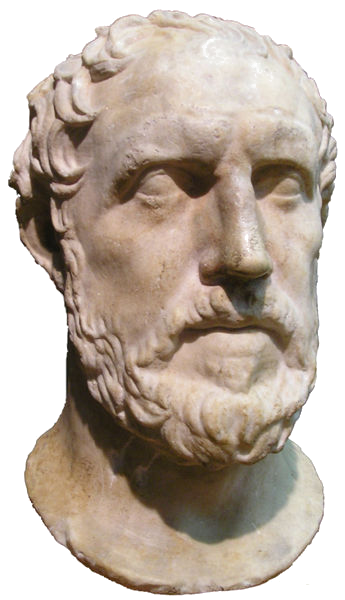
\includegraphics[width=0.9\textwidth]{../FIGS//Thucydides-bust}
\end{center}
\end{minipage}
}


\maxFrameImage{../FIGS/trade_routes_1212AD}\maxFrameImage{../FIGS/map-black-death.jpg}

{
\backgroundImage{../FIGS/Yersinia_pestis_fluorescent.jpeg}
\begin{frame}{The Black Death: a few facts}
	\begin{itemize}
		\item First of the middle ages plagues to hit Europe
		\vfill
		\item Affected Afro-Eurasia from 1346 to 1353
		\vfill
		\item Europe 1347-1351
		\vfill
		\item Killed 75-200M in Eurasia \& North Africa
		\vfill
		\item Killed 30-60\% of European population
	\end{itemize}
\end{frame}
}

{
\backgroundImage{../FIGS/Nuremberg-chronicles-Dance-of-Death-CCLXIIIIv.jpg}
\begin{frame}{Plague control measures}
	\begin{itemize}
		\item Lazzarettos of Dubrovnik 1377 (30 days)
		\vfill
		\item Quarantena of Venice 1448 (40 days)
		\vfill
		\item Isolation of known or suspected cases as well as persons who had been in contact with them, at first for 14 days and gradually increased to 40 days
		\vfill
		\item Improvement of sanitation: development of pure water supplies, garbage and sewage disposal, food inspection
		\vfill
		\item Find and kill a snake, chop it into pieces and rub the various parts over swollen buboes. (Snake, synonymous with Satan, was thought to draw the disease out of the body as evil would be drawn to evil)
	\end{itemize}
\end{frame}
}

\maxFrameImage{../FIGS/Snow-cholera-map-inverted}

\begin{frame}{Pathogen spread has evolved with mobility}
	\begin{itemize}
		\item Pathogens travel along trade routes
		\vfill
		\item In ancient times, trade routes were relatively easy to comprehend
		\vfill
		\item With acceleration and globalization of mobility, things have changed
	\end{itemize}
\end{frame}

\maxFrameImage{../FIGS/rail-map-Europe}
\maxFrameImage{../FIGS/rail-map-China}



% ![bg contain](https://www.cmaj.ca/content/cmaj/182/6/579/F2.large.jpg)

% ---

% ![bg contain](https://raw.githubusercontent.com/julien-arino/presentations/main/FIGS/transportation/passengers_transported_worldwide.png)

% ---

{
\backgroundImage{../FIGS/af3c1e4a-9ca9-4caa-8cbb-7f4f34c9ac88}
% Image from https://slate.com/news-and-politics/2019/02/trump-border-wall-nogales-arizona-razor-wire.html
\begin{frame}{Fragmented jurisdictional landscapes}
	\begin{itemize}
		\item  Political divisions (jurisdictions): nation groups (e.g., EU), nations, provinces/states, regions, counties, cities..
		\vfill
		\item Travel between jurisdictions can be complicated or impossible
		\vfill
		\item Data is integrated at the jurisdictional level
		\vfill
		\item Policy is decided at the jurisdictional level
	\end{itemize}
\end{frame}
}

\begin{frame}{Why mobility is important in the context of health}
	\begin{quote}
		All migrants/travellers carry with them their "health history"
	\end{quote}
	\vfill
	\begin{itemize}
		\item latent and/or active infections (TB, H1N1, polio)
		\item immunizations (schedules vary by country)
		\item health/nutrition practices (KJv)
		\item treatment methods (antivirals)
	\end{itemize}
	\vfill
	\begin{quote}
		Pathogens ignore borders and politics
	\end{quote}
\end{frame}

\maxFrameImage{../FIGS/SARS_countries_with_time}

\maxFrameImage{../FIGS/polio-vaccine-coverage-2004_blackBG}
\maxFrameImage{../FIGS/polio-cases-2000-2005-noNGA_blackBG}
\maxFrameImage{../FIGS/polio-cases-2000-2005-withNGA_blackBG}
\maxFrameImage{../FIGS/nejmp068200_f1.jpeg}

%%%%%%%%%%%%%%%%%%%
%%%%%%%%%%%%%%%%%%%
\subsection{Spatial aspects in animal diseases}

\begin{frame}{Diseases in wild animals}
	Spread typically follows travelling wave patterns
	\vfill
	Next slides: cases of rabies 
\end{frame}

\maxFrameImage{../FIGS/rabies_1990-noBG}
\maxFrameImage{../FIGS/rabies_2000-noBG}
\maxFrameImage{../FIGS/rabies_2010-noBG}

\begin{frame}{Diseases in livestock}
	Situation is more complicated
\end{frame}



%%%%%%%%%%%%%%%%%%%
%%%%%%%%%%%%%%%%%%%
\subsection{Foot-and-mouth disease}

%%%%%%%%%%%%%%%%%%%
\maxFrameImage{../FIGS/JamalBelsham-FMD-geography-inverted}
\maxFrameImage{../FIGS/JamalBelsham-FMD-control-inverted}
\maxFrameImage{../FIGS/GrubmanBaxt-FMD-spread-panAsian-inverted}
\maxFrameImage{../FIGS/Rweyemamu_etal-FMD-patterns-spread-old-world-inverted}

%%%%%%%%%%%%%%%%%%%
\maxFrameImage{../FIGS/Gibbens_etal-FMD-UK2001-epi-cover-inverted}
\maxFrameImage{../FIGS/Gibbens_etal-FMD-UK2001-epi-cases}
\maxFrameImage{../FIGS/Gibbens_etal-FMD-UK2001-epi-infected-premises2-inverted}
\maxFrameImage{../FIGS/Gibbens_etal-FMD-UK2001-epi-infected-premises1-inverted}
\maxFrameImage{../FIGS/Gibbens_etal-FMD-UK2001-epi-cumulative-incidence-inverted}
\maxFrameImage{../FIGS/Gibbens_etal-FMD-UK2001-epi-movement-inverted}

\begin{frame}{2001 FMD epidemic in the UK}
	\footnotesize
	\begin{itemize}
		\item Early February -- Disease likely to have entered the UK
		\item 19th February -- Foot-and-mouth disease first suspected
		\item 20th February -- Foot-and-mouth disease confirmed
		\item 23rd February -- Culling initiated of Infected Premises  (IP) and Dangerous Contacts (DC). Movement restrictions are brought into force
		\item 15th March -- Sheep, goats and pigs within 3km of an IP in Lockerbie, Carlisle and Solway are targeted for culling
		\item 23rd March -- Contiguous Premises (CPs) are included in the cull
		\item 26th March -- Epidemic reaches its maximum with 54 cases in one day
		\item 27th March -- 3km cull begins in the Penrith valley, Cumbria
		\item 29th March -- 24/48 hour policy begins, in which IPs are slaughtered within 24 hours, and DCs and CPs are culled within 48 hours
		\item 14th April -- 3km cull in Cumbria reaches its height
		\item 26th April -- Sheep, pigs and especially cattle from farms with high biosecurity may be exempt from culls
		\item 10th May -- First case reported in the Settle area
		\item 20th June -- First day with no reported cases
	\end{itemize}
\end{frame}


%%%%%%%%%%%%%%%%%%%
%%%%%%%%%%%%%%%%%%%
\subsection{Avian influenza}
\begin{frame}
	\begin{itemize}
		\item Avian Influenza global concern because it involves multiple bird species, both wild and livestock
		\vfill
		\item The thing with wild birds is that they fly... :)
	\end{itemize}
\end{frame}

\maxFrameImage{../FIGS/mm-birds3-inverted}

%%%%%%%%%%%%%%%%%%%
\maxFrameImage{../FIGS/Sonnberg_etal-HPAI-natural-history-interactions-inverted}

%%%%%%%%%%%%%%%%%%%
\maxFrameImage{../FIGS/LupianiReddy-AI-table-inverted}

%%%%%%%%%%%%%%%%%%%
\maxFrameImage{../FIGS/Kilpatrick_etal-global-spread-H5N1-cover-inverted}
\maxFrameImage{../FIGS/Kilpatrick_etal-global-spread-H5N1-philo-inverted}
\maxFrameImage{../FIGS/Kilpatrick_etal-global-spread-H5N1-map}
\maxFrameImage{../FIGS/Kilpatrick_etal-global-spread-H5N1-world}

%%%%%%%%%%%%%%%%%%%
\maxFrameImage{../FIGS/Napp_etal-H5N8-Europe-cover-inverted}
\maxFrameImage{../FIGS/Napp_etal-H5N8-Europe-spatial-distrib}
\maxFrameImage{../FIGS/Napp_etal-H5N8-Europe-timeline-map}
\maxFrameImage{../FIGS/Napp_etal-H5N8-Europe-table-inverted}
\maxFrameImage{../FIGS/Napp_etal-H5N8-Europe-pct-outbreaks-table-inverted}

%%%%%%%%%%%%%%%%%%%
\maxFrameImage{../FIGS/H5N8-Science-cover-inverted}
\maxFrameImage{../FIGS/H5N8-Science-maps}


%%%%%%%%%%%%%%%%%%%
%%%%%%%%%%%%%%%%%%%
\section{Metapopulation models}

\frame{\frametitle{What are metapopulations?}
Metapopulations are \emph{populations} of \emph{populations}.
\vfill
Two main types of metapopulation models:
\begin{itemize}
\item \emph{patch occupancy models}. Describe whether a location is \emph{occupied} by a species or not. Depends on the occupancy of neighboring or connected locations. Dynamics describes the number of occupied locations
\item Models with \emph{explicit movement}. Movement between locations is described explicitly. In each location, a set of differential equations describes the dynamics of the populations present
\end{itemize}
}

{
\backgroundImage{../FIGS/DirichletEurope}
\frame{\frametitle{What is a location?}
A \emph{location} is a unit (typically geographical) within which the population is considered homogeneous
\begin{itemize}
\item city
\item region
\item country
\item but also, location where a given species lives (for example, forest, swamp, etc.)
\end{itemize}
\vfill
Locations may or may not overlap
}}

%%%%%%%%%%%%%%%%%%%
%%%%%%%%%%%%%%%%%%%
\subsection[Implicit movement]{Metapopulations \`a la Levins}

\begin{frame}{A model of Richard Levins (1969)}
    R. Levins. \href{https://doi.org/10.1093/besa/15.3.237}{Some Demographic and Genetic Consequences of Environmental Heterogeneity for Biological Control}. 
    Bulletin of the Entomological Society of America \textbf{15}(3): 237-240 (1969)
    \vfill
    Cited 4,400+ times, numerous higher order ``offspring''
	\vfill
	Quickly evolved to include prey-predators or competition systems
\end{frame}

\begin{frame}{The Levins model}
Rate of change of \# of local populations $P$:
\begin{equation}
P' = \beta P \left( 1 - \frac{P}{T} \right) -\mu P
\label{eq:Levins}
\end{equation}
$\beta$ immigration rate between \emph{locations}, $T$ total number of locations and $\mu$ extinction rate of local populations
\vfill
Ecologists \& mathematicians think of patches differently. For mathematicians, typically, one place in space. To be clear, in the remainder of these slides, I will speak of \emph{locations}
\end{frame}

\begin{frame}{Metapopulations with implicit movement}
    Same philosophy as the Levins model
    \vfill
    \begin{itemize}
        \item There is a set $\P$ of locations called \emph{locations}
        \item Each location $p\in\P$ has an internal dynamics $x_p'=f_p(x_p)$, where $x_p\in\IR_+^{n_p}$ and $f_p:\IR^{n_p}\to \IR^{n_p}$
        \item No flow of individuals between locations
        \item The influence of location $q\neq p$ on $p$ is described through a function $g_{qp}(x_p,x_q)$, where $x_q\in\IR^{n_q}$ and $g_p:\IR^{n_p}\times\IR^{n_q}\to\IR^{n_p}$
    \end{itemize}
    \vfill
    So the population in location $p\in\P$ has dynamics
    \begin{equation}\label{eq:metapop_implicit_mvt_generic}
        x_p' = f_p(x_p)
        +\sum\dind{q\in\P}{q\neq p}
        g_{qp}(x_p,x_q)
    \end{equation}
\end{frame}

%%%%%%%%%%%%%%%%%%%
%%%%%%%%%%%%%%%%%%%
\subsection[Explicit movement]{Metapopulations \`a la Levin}

\begin{frame}{Levins-type vs Explicit movement}
	Levins model and its offspring: movement is implicit
	\[
	P' = \beta P \left( 1 - \frac{P}{T} \right) -\mu P
	\]
	$\beta$ immigration rate between locations incorporates geography
	\vfill
	Sometimes we have explicit movement information or want to incorporate known spatial information $\implies$ models with explicit movement 
	\vfill Levin (1974) 
\end{frame}

\frame{\frametitle{Metapopulations with explicit movement}
	Split continuous space into $N$ discrete geographical locations (\emph{ptatches})
	\vfill
	Each location contains \textbf{compartments} (homogeneous groups of individuals). E.g., preys, predators, etc. 
	\vfill
	Here, we consider a single compartment, the \emph{species of interest}, with no further compartmentalisation
	\vfill
	Individuals \emph{may} move between locations; $m_{qp}\geq 0$ rate of movement of individuals from location $p=1,\ldots,N$ to location $q=1,\ldots,N$
	\vfill
}

\frame{\frametitle{Explicit movement (focus on $P_1$)}
	\begin{center}		
	\begin{tikzpicture}[auto, %node distance = 2cm, auto,
	cloud/.style={minimum width={width("N-1")+2pt},
		draw, ellipse,fill=red!70}]
	\node [cloud] (P1) {$P_1$};
	\node [cloud, above right=of P1] (P2) {$P_2$};
	\node [cloud, right=of P1] (P3) {$P_3$};
	\node [cloud, below right=of P1] (P4) {$P_4$};
	\node [cloud, below=of P1] (P5) {$P_5$};
	\node [cloud, below left=of P1] (P6) {$P_6$};
	\node [cloud, above left=of P1] (Pk) {$P_k$};
	%% Outflows
	\path [line, very thick, blue] (P1) to [bend left = 20] node [midway, left] (TextNode) {$m_{21}$} (P2);
	\path [line, very thick, blue] (P1) to [bend left = 20] node [midway, below] (TextNode) {$m_{31}$} (P3);
	\path [line, very thick, blue] (P1) to [bend left = 20] node [pos=0.9, right] (TextNode) {$m_{51}$} (P5);
	\path [line, very thick, blue] (P1) to [bend left = 20] node [midway, right] (TextNode) {$m_{61}$} (P6);
	\path [line, very thick, blue, densely dashed] (P1) to [bend left = 20] node [midway, left] (TextNode) {$m_{k1}$} (Pk);
	%% Inflows
	\path [line, very thick, red] (P2) to [bend left = 20] node [midway, right] (TextNode) {$m_{12}$} (P1);
	\path [line, very thick, red] (P4) to [bend left = 20] node [right] (TextNode) {$m_{14}$} (P1);
	\path [line, very thick, red] (P6) to [bend left = 20] node [left] (TextNode) {$m_{16}$} (P1);
	\path [line, very thick, red, densely dashed] (Pk) to [bend left = 20] node [right, pos=0.1] (TextNode) {$m_{1k}$} (P1);
	\end{tikzpicture}
	\end{center}
	\[
	P_1' = {\red \sum_{\substack{j=1\\j\neq 1}}^{N}m_{1j}P_j}
	{\blue -P_1\sum_{\substack{j=1\\j\neq 1}}^{N}m_{j1}}
	\]
	or
	\[
	P_1' = \sum_{j=1}^{N} m_{1j}P_j
	\textrm{ assuming }
	m_{11}=-\sum_{\substack{j=1\\j\neq 1}}^{N} m_{j1}
	\]
}


%%%%%%%%%%%%%%%%%%%
%%%%%%%%%%%%%%%%%%%
\subsection{The graph setting}


\begin{frame}\frametitle{Graph setting}
Suppose
\begin{itemize} 
\item $|\P|$ locations, vertices in a (directed) graph $\G$
\item Each location contains a certain number of compartments belonging to a common set $\C$ of compartments
\item Arcs of $\G$ represent the possibility for a given compartment to move between two locations; any two locations are connected by a maximum of $|\C|$ edges
\end{itemize}
\vfill
Graph is a digraph: movement is not always symmetric
\end{frame}


\begin{frame}
$\G=(\P,\A)$ is multi-digraph, where 
\begin{itemize}
	\item $\P$ is the set of vertices (locations)
	\item $\A$ is the set of arcs, i.e., an ordered multiset of pairs of elements of $\P$
\end{itemize}
\vfill
Any two vertices $X,Y\in\P$ are connected by at most $|\C|$ arcs from $X$ to $Y$ and at most $|\C|$ arcs from $Y$ to $X$
\vfill
Because there are $|\C|$ compartments and movements are compartment-specific, we also define, for all $c\in\C$, $\P_c$ and $\A_c$ as well as the compartment-specific digraphs $\G^c=(\P_c,\A_c)$
\end{frame}


\frame{\frametitle{Connection matrix}
For a given compartment $c\in\C$, a \emph{connection matrix} can be associated to the digraph $\G_c$
\vfill
This is the \textbf{adjacency matrix} of $\G_c$, but we emphasize the reason why we use $\G_c$ by using the term \emph{connection}
\vfill
Choosing an ordering of elements of $\P$, the $(i,j)$ entry of the $|\P|\times|\P|$-matrix $\N_c=\N_c(\G_c)$ is one if $R^c(P_i,P_j)$ and zero otherwise, i.e., if $P_i$ has no direct access to $P_j$
\vfill
For convenience, the ordering of the locations is generally assumed the same for all compartments
}

\frame{\frametitle{Strongly connected multi-digraph}
\begin{definition}[Strongly connected components]
For a given compartment $s$, the \textbf{strongly connected components} (or \textbf{strong components}, for short) are such that, for all locations $X,Y$ in a strong component, compartment $s$ in $X$ has access to $Y$
\end{definition}
\vfill
\begin{definition}[Strong connectedness for a compartment]
The multi-digraph is strongly connected for compartment $c$ if all locations belong to the same strong component of $\G_c$
\end{definition}
}

\frame{\frametitle{Srong connectedness and irreducibility}
\begin{definition}[Reducible/irreducible matrix]
	\label{def:reducible_irreducible_matrix}
	A matrix $A$ is \textbf{reducible} if there exists a permutation matrix $P$ such that $P^TAP$ is block upper triangular. A matrix that is not reducible is \textbf{irreducible}
\end{definition}
\vfill
Matrix $A\in\IF^{n\times n}$ is irreducible if for all $i,j=1,\ldots,n$, there exists $k$ such that $a_{ij}^k>0$, where $a_{ij}^k$ is the $(i,j)$-entry in $A^k$
\vfill
\begin{theorem}
	Strong connectedness $\Leftrightarrow$ \textbf{irreducibility} of the connection matrix $\mathcal{C}_c$
\end{theorem}
}



%%%%%%%%%%%%%%%%%%%
%%%%%%%%%%%%%%%%%%%
\subsection{Generic model}

\frame{\frametitle{Notation}
\begin{itemize}
	\item $N_{cp}(t)$ number of individuals of compartment $c$ in location $p$ at time $t$
	\vfill
	\item $\bN_c=\left(N_{c1},\ldots,N_{c|\P|}\right)^T$ distribution of individuals of compartment $c\in\C$ among the different locations 
	\vfill
	\item $N^p=\left(N_1^p,\ldots,N_{|\P|}^p\right)^T$ composition of the population in location $p\in\P$
\end{itemize}
}

\frame{\frametitle{Metapopulation models with linear movement}
Use a linear autonomous movement operator
\vfill
Then, for a given compartment $c\in\C$ and in a given location $p\in\P$
\[
	N_{cp}'=f_{cp}(N^p)
	+\sum\dind{q\in\P}{q\neq p}m_{cpq}N_{cq} 
	-\left(\sum\dind{q\in\P}{q\neq p}m_{cqp}\right)N_{cp}
\]
where $m_{cpq}$ rate of movement of individuals in compartment $c\in\C$ from location $q\in\P$ to location $p\in\P$
}

\begin{frame}{A more compact notation}
	To make 
	\[
		N_{cp}'=f_{cp}(N^p)
		+\sum\dind{q\in\P}{q\neq p}m_{cpq}N_{cq} 
		-\left(\sum\dind{q\in\P}{q\neq p}m_{cqp}\right)N_{cp}
	\]
	more compact, denote the rate of leaving location $p$ as
	\begin{equation}
		m_{cpp} = -\sum\dind{q\in\P}{q\neq p}m_{cqp}
	\end{equation}
	Then
	\begin{equation}\label{eq:general_metapop_linear_migration}
		N_s'=f_{cp}(N^p)+\sum_{q\in\P}m_{cpq}N_{cq}
	\end{equation}
\end{frame}

\begin{frame}{Vector form of the system}
For compartment $c\in\C$,
\begin{equation}\label{eq:general_metapop}
\bN_c'=f(\bN)+\mathcal{M}_c\bN_c
\end{equation}
with
\begin{equation}\label{eq:movement_matrix}
\mathcal{M}_c =
\begin{pmatrix}
-\sum\limits_{k\in\P}m_{ck1} & m_{c12} & \cdots & m_{c1|\P|} \\
& & & \\
m_{c|\P|1} & m_{c|\P|2} & \cdots & -\sum\limits_{k\in\P}m_{ck|\P|}
\end{pmatrix}
\end{equation}
\end{frame}


%%%%%%%%%%%%%%%%%%
%%%%%%%%%%%%%%%%%%
\subsection{The movement matrix}

\begin{frame}{Definitions and notation for matrices}
\begin{itemize}
	\item $M\in\mathbb{R}^{n\times n}$ a square matrix with entries denoted $m_{ij}$
	\vfill
	\item $M\geq\mathbf{0}$ if $m_{ij}\geq 0$ for all $i,j$ (could be the zero matrix); $M>\mathbf{0}$ if $M\geq\mathbf{0}$ and $\exists i,j$ with $m_{ij}>0$; $M\gg\mathbf{0}$ if $m_{ij}>0$ $\forall i,j=1,\ldots,n$. Same notation for vectors
	\vfill
	\item $\sigma(M)=\{\lambda\in\mathbf{C}; M\lambda=\lambda\mathbf{v}, \mathbf{v}\neq\mathbf{0}\}$ \textbf{spectrum} of $M$
	\vfill
	\item $\rho(M)=\max_{\lambda\in\sigma(M)}\{|\lambda|\}$ \textbf{spectral radius}
	\vfill
	\item $s(M)=\max_{\lambda\in\sigma(M)}\{\Re(\lambda)\}$ \textbf{spectral abscissa} (or \textbf{stability modulus})
	\vfill
	\item $M$ is an \textbf{M-matrix} if it is a \textbf{Z-matrix} ($m_{ij}\leq 0$ for $i\neq j$) and $M = s\mathbb{I}-A$, with $A\geq 0$ and $s\geq \rho(A)$
\end{itemize}
\end{frame}

\begin{frame}{The movement matrix}
	The matrix
	\begin{equation}\tag{\ref{eq:movement_matrix}}
		\mathcal{M}_c =
		\begin{pmatrix}
		-\sum\limits_{k\in\P}m_{ck1} & m_{c12} & \cdots & m_{c1|\P|} \\
		& & & \\
		m_{c|\P|1} & m_{c|\P|2} & \cdots & -\sum\limits_{k\in\P}m_{ck|\P|}
		\end{pmatrix}
	\end{equation}
	is the \textbf{movement matrix}
	\vfill
	It plays an extremely important role in the analysis of metapopulation systems, so we'll spend some time discussing its properties
	\vfill
$\mathcal{M}_c$ describes
\begin{itemize} 
\item existence of connections
\item when they exist, their ``intensity''
\end{itemize}
\end{frame}

\begin{frame}{Properties of the movement matrix $\M$}
	First, remark $-\M_c$ is a Laplacian matrix
	\vfill
	\begin{lemma}\label{lemma:behaviour_Mc}
		\begin{enumerate}
			\item $0\in\sigma(\M)$ corresponding to left e.v. $\11^T$ \hfill[$\sigma$ spectrum]
			\item $-\M$ is a singular M-matrix
			\item $0=s(\M)\in\sigma(\M)$ \hfill[$s$ spectral abscissa]
			\item If $\M$ irreducible, then $s(\M)$ has multiplicity 1
		\end{enumerate}
	\end{lemma}
	\vfill
	For complete proof of Lemma~\ref{lemma:behaviour_Mc} and Proposition~\ref{prop:behaviour_Mc} (next page), see \href{http://dx.doi.org/10.1007/s11538-019-00593-1}{Arino, Bajeux \& Kirkland, BMB 2019}
\end{frame}

\begin{frame}
	\begin{proposition}[$D$ a diagonal matrix]
		\label{prop:behaviour_Mc}
		\begin{enumerate}
			\item $s(\M+d\II)=d$, $\forall d\in\IR$
			\item $s(\M+D)\in\sigma(\M+D)$ associated to $\bv>\b0$. If $\M$ irreducible, $s(\M+D)$ has  multiplicity 1 and is associated to $\bv\gg \b0$
			\item If $\diag (D)\gg \b0$, then $D-\M$ invertible M-matrix and $(D-\M)^{-1}> \b0$
			\item $\M$ irreducible and $\diag(D)>\b0$ $\Longrightarrow$ $D-\M$ nonsingular irreducible M-matrix and $(D-\M)^{-1}\gg \b0$		
		\end{enumerate}
	\end{proposition}
\end{frame}


%%%%%%%%%%%%%%%%%
%%%%%%%%%%%%%%%%%
\subsection{Behaviour of the mobility component}
\frame{\frametitle{Behaviour of the mobility component}
Assume no within-location dynamics, just movement. Then \eqref{eq:general_metapop} takes the form
\begin{equation}\label{eq:mobility_compartment}
	\bN_c' = \mathcal{M}_c\bN_c
\end{equation}
\vfill
\begin{theorem}\label{th:GAS_metapop1}
For a given compartment $c\in\C$, suppose that the movement matrix $\M_c$ is irreducible. Then for any $\bN_c(0)>0$, \eqref{eq:mobility_compartment} satisfies
\[
\lim_{t\to\infty}\bN_c(t)=\bN_c^\star\gg 0
\]
\end{theorem}
\vfill
Note that $\bN_c^\star$ depends on $\nbOne^T\bN_c(0)$
}



\begin{frame}{Reduction to total population per location}
Let 
\[
	T_p = \sum_{c\in\C}N_{cp}
\]
be the total population in location $p$
\vfill
It is often posssible to obtain, in each location $p\in\P$, an equation for the evolution of the total population that takes the form
\begin{equation}\label{eq:dT_total_population}
	T_p' = 
	D_p(T_p)+\sum_{c\in\C}\sum_{q\in\P}m_{cpq}N_{cq}
\end{equation}
where $D_p(T_p)$ describes the demography in location $p$
\end{frame}

\begin{frame}{Nature of the demography}
	Most common types of demographic functions
	\begin{itemize}
		\item $D_p(T_p)=b_p-d_pT_p$ (asymptotically constant population)
		\item $D_p(T_p)=b_pT_p-d_pT_p$ 
		\item $D_p(T_p)=d_pT_p-d_pT_p=0$ (constant population)
		\item $D_p(T_p)=r_pT_p(1-T_p/K_p)$ (logistic demography)
	\end{itemize}
	\vfill
	In what follows, assume 
	\begin{equation}\label{eq:demography_function}
		D_p(T_p)=b_p-d_pT_p
	\end{equation}
\end{frame}

\begin{frame}{Vector / matrix form of the equation}
Assuming demography is of the form \eqref{eq:demography_function}, write \eqref{eq:dT_total_population} in vector form
\begin{equation}\label{sys:dN_general} 
	\mathbf{T}'=\mathbf{b}-\bd\bT+\sum_{c\in\C}\mathcal{M}_c\bN_{c}	
\end{equation}
where 
\begin{itemize}
	\item $\mathbf{b}=(b_1,\ldots,b_{|\mathcal{P}|})^T\in\IR^{|\P|}$
	\item $\mathbf{T}=(T_1,\ldots,T_{|\mathcal{P}|})^T\in\IR^{|\P|}$
	\item $\mathbf{N}=(N_{c1},\ldots,N_{c{|\mathcal{P}|}})^T\in\IR^{|\P|}$
	\item $\bd=\mathsf{diag}\left(d_1,\ldots,d_{|\mathcal{P}|}\right)\in\IR^{|\mathcal{P}|\times|\mathcal{P}|}$
	\item $\mathcal{M}_c\in\IR^{|\mathcal{P}|\times|\mathcal{P}|}$
\end{itemize}

\end{frame}


\begin{frame}{The nice case}
Suppose movement rates \textbf{equal for all compartments}, i.e.,
$$
\M_c\equiv\M
$$
\vfill
Then
\begin{align}
\bT' &= \bb-\bd\bT+\M\sum_{c\in\C}\bN_{c} \nonumber \\
&= \bb-\bd\bT+\M\bT \label{sys:pSLIRS_toy_dN}
\end{align}
\end{frame}


\begin{frame}{Equilibria}
$$
\begin{aligned}
\bT'=\b0 &\Leftrightarrow \mathbf{b}-\bd\mathbf{T}+\mathcal{M}\mathbf{T}=\mathbf{0} \\
&\Leftrightarrow (\bd-\mathcal{M})\mathbf{T}=\mathbf{b} \\
&\Leftrightarrow \mathbf{T}^\star=(\bd-\mathcal{M})^{-1}\mathbf{b}
\end{aligned}
$$
given, of course, that $\bd-\mathcal{M}$ (or, equivalently, $\mathcal{M}-\bd$) is invertible.. 
\vfill
Is it?
\end{frame}

\begin{frame}{Nonsingularity of $\mathcal{M}-\bd$}
Using the spectrum shift of Theorem~\ref{prop:behaviour_Mc}{(1)}
\[
s\left(\mathcal{M}-\min_{p\in\mathcal{P}}d_p\right)=-\min_{p\in\mathcal{P}}d_p
\]
This gives a constraint: for total population to behave well (in general, we want this), we \emph{must assume all death rates are positive}
\vfill
Assume they are (in other words, assume $\bd$ nonsingular). Then $\mathcal{M}-\bd$ is nonsingular and $\bT^\star=(\bd-\mathcal{M})^{-1}\mathbf{b}$ unique
\end{frame}


\begin{frame}{Behaviour of the total population}
\framesubtitle{Equal irreducible movement case}
$\mathbf{T}^\star=(\bd-\mathcal{M})^{-1}\mathbf{b}$ attracts solutions of
$$
\mathbf{T}'=\mathbf{b}-\bd\mathbf{T}+\mathcal{M}\mathbf{T}=:f(\mathbf{T})
$$
\vfill
Indeed, we have
$$
Df=\mathcal{M}-\bd
$$
\vfill
Since we now assume that $\bd$ is nonsingular, we have by Theorem~\ref{prop:behaviour_Mc}{(1)} that $s(\mathcal{M}-\min_{p\in\mathcal{P}}d_p)=-\min_{p\in\mathcal{P}}d_p<0$
\vfill
$\mathcal{M}$ irreducible $\rightarrow$ $\mathbf{T}^\star\gg 0$ (provided $\mathbf{b}>\mathbf{0}$, of course)
\end{frame}




%%%%%%%%%%%%%%%%%%%
%%%%%%%%%%%%%%%%%%%
\subsection{A few sample models}


\frame{\frametitle{The toy SLIRS model in patches}
\begin{center}
	\begin{tikzpicture}[scale=1, every node/.style={transform shape},
		auto, %node distance = 2cm, auto,
		box/.style={minimum width={width("N-1")+2pt},
			draw, rectangle,fill=red!70}]
		%% States
		\node [box] at (0,2) (S) {$S$};
		\node [box] at (2,2) (L) {$L$};
		\node [box] at (4,2) (I) {$I$};
		\node [box] at (6,2) (R) {$R$};
		%% Flows
		\path [line, thick] (-1.5,2) to node [midway, above] (TextNode) {$b$} (S);
		\path [line, thick] (S) to node [midway, above, sloped] (TextNode) {$\Phi$} (L);
		\path [line, thick] (L) to node [midway, above] (TextNode) {$\varepsilon L$} (I);
		\path [line, thick] (I) to node [sloped, midway, above] (TextNode) {$\gamma I$} (R);
		\draw [>=latex,->, thick, rounded corners] (R) -- +(0,0.75) -- ++(-6,0.75) node[midway, above] {$\nu R$} -- (S);
		\path [line, thick] (S) to node [midway, right] (TextNode) {$dS$} ++(0,-1);
		\path [line, thick] (L) to node [midway, right] (TextNode) {$dL$} ++(0,-1);
		\path [line, thick] (I) to node [midway, right] (TextNode) {$(d+\delta)I$} ++(0,-1);
		\path [line, thick] (R) to node [midway, right] (TextNode) {$dR$} ++(0,-1);
	\end{tikzpicture}
\end{center}
\begin{subequations}\label{sys:SLIRS}
\begin{align}
S' &= b+\nu R-\Phi-dS \\
L' &= \Phi-(\varepsilon+d)L\\
I' &= \varepsilon L-(\gamma+d+\delta)I\\
R' &= \gamma I-(\nu+d)R
\end{align}
\end{subequations}
$\Phi$ force of infection. Depends on $S,I$, possibly $N$. In general
\[
\Phi=\beta(N)\phi(S,I)
\] 

Mass action, $\Phi=\beta SI$, proportional incidence, $\Phi=\beta SI/N$
}



\frame{\frametitle{$|\mathcal{P}|$-SLIRS model}
\begin{subequations}
	\label{sys:pSLIRS}
	\begin{align}
		S_{p}' &=b_p+\nu_pR_p-\Phi_p-d_pS_p 
		\color{red}{+\textstyle{\sum_{q\in\mathcal{P}}} m_{Spq}S_{q}} 
		\label{sys:pSLIRS_dS} \\
		L_{p}' &=\Phi_p-\left( \varepsilon_{p}+d_{p}\right)L_{p}
		\color{red}{+\textstyle{\sum_{q\in\mathcal{P}}} m_{Lpq}L_{q}} 
		\label{sys:pSLIRS_dL} \\
		I_{p}' &=\varepsilon_pL_p-(\gamma_p+d_p)I_p
		\color{red}{+\textstyle{\sum_{q\in\mathcal{P}}} m_{Ipq}I_{q}} 
		\label{sys:pSLIRS_dI} \\
		R_{p}' &=\gamma _{p}I_{p}-\left(\nu_{p}+d_{p}\right)R_{p}
		\color{red}{+\textstyle{\sum_{q\in\mathcal{P}}} m_{Rpq}R_{q}} 
		\label{sys:pSLIRS_dR} 
	\end{align}
	with incidence 
	\begin{equation}
		\Phi_p=\beta_p\frac{S_pI_p}{N_p^{q_p}},\qquad q_p\in\{0,1\}
		\label{sys:pSLIRS_incidence} 
	\end{equation}
\end{subequations}	
}

\begin{frame}
\frametitle{$|\S|\;|\P|$-SLIRS (multiple species)}
$p\in\P$ and $s\in\mathcal{S}$ (a set of species)
\vfill
\begin{subequations}
	\label{sys:spSLIRS}
	\begin{align}
		S_{sp}' &= b_{sp}+\nu_{sp}R_{sp}-\Phi_{sp}-d_{sp}S_{sp}
		\color{red}{+\textstyle{\sum_{q\in\mathcal{P}}} m_{Sspq}S_{sq}} 
		\label{sys:spSLIRS_dS} \\
		L_{sp}' &= \Phi_{sp}-(\varepsilon_{sp}+d_{sp})L_{sp}
		\color{red}{+\textstyle{\sum_{q\in\mathcal{P}}}m_{Lspq}L_{sq}}
		\label{sys:spSLIRS_dL} \\
		I_{sp}' &= \varepsilon_{sp}L_{sp}-(\gamma_{sp}+d_{sp})I_{sp}
		\color{red}{+\textstyle{\sum_{q\in\mathcal{P}}} m_{Ispq}I_{sq}}
		\label{sys:spSLIRS_dI} \\
		R_{sp} &= \gamma _{sp}I_{sp}-(\nu_{sp}+d_{sp})R_{sp}
		\color{red}{+\textstyle{\sum_{q\in\mathcal{P}}} m_{Rspq}R_{sq}} 
		\label{sys:spSLIRS_dR} 
	\end{align}
	with incidence
	\begin{equation}
	\Phi_{sp}=\sum_{k\in\mathcal{S}}\beta_{skp}\frac{S_{sp}I_{kp}}{N_p^{q_p}},\qquad q_p\in\{0,1\}
	\label{sys:spSLIRS_incidence} 
	\end{equation}
\end{subequations}
\vfill
{\tiny
\begin{itemize}
\setlength{\itemsep}{-5pt}
\item JA, Davis, Hartley, Jordan, Miller \& PvdD. \href{https://julien-arino.github.io/assets/pdf/papers/2005_ArinoDavisHartleyJordanMillerPvdD-MMB22.pdf}{A multi-species epidemic model with spatial dynamics}. \emph{Mathematical Medicine and Biology} \textbf{22}(2):129-142 (2005)\newline 
\item JA, Jordan \& PvdD. \href{https://julien-arino.github.io/assets/pdf/papers/2007_ArinoJordanPvdD-MBS206.pdf}{Quarantine in a multi-species epidemic model with spatial dynamics}. \emph{Mathematical Biosciences} \textbf{206}(1):46-60 (2007)
\end{itemize}}
\end{frame}

\frame{
\frametitle{$|\P|^2$-SLIRS (residents-travellers)}
\begin{subequations}
	\label{sys:ppSLIRS}
	\begin{align}
		S_{pq}' =& 
		b_{pq}+\nu_{pq} R_{pq}-\Phi_{pq}-d_{pq}S_{pq} \color{red}{+\textstyle{\sum_{k\in\mathcal{P}}} m_{Spqk}S_{pk}} 
		\label{sys:ppSLIRS_dS} \\
		L_{pq}' =& \Phi_{pq}
		-(\varepsilon_{pq}+d_{pq})L_{pq}
		\color{red}{+\textstyle{\sum_{k\in\mathcal{P}}} m_{Lpqk}L_{pk}} 
		\label{sys:ppSLIRS_dL} \\
		I_{pq}' =& \varepsilon_{pq} L_{pq}
		-(\gamma_{pq}+d_{pq})I_{pq}
		\color{red}{+\textstyle{\sum_{k\in\mathcal{P}}} m_{Ipqk}I_{pk}} 
		\label{sys:ppSLIRS_dI} \\
		R_{pq}' =& \gamma_{pq} I_{pq}
		-(\nu_{pq}+d_{pq})R_{pq}
		\color{red}{+\textstyle{\sum_{k\in\mathcal{P}}} m_{Rpqk}R_{pk}}
		\label{sys:ppSLIRS_dR} 
	\end{align}
	with incidence
	\begin{equation}
		\Phi_{pq}=\sum_{k\in\mathcal{P}}\beta_{pqk}\frac{S_{pq}I_{kq}}{N_p^{q_q}},\qquad q_q=\{0,1\}
		\label{sys:ppSLIRS_incidence} 
	\end{equation}
\end{subequations}

\vfill
{\tiny
\begin{itemize}
%\setlength{\itemsep}{-5pt}
\item Sattenspiel \& Dietz. \href{https://doi.org/10.1016/0025-5564(94)00068-B}{A structured epidemic model incorporating geographic mobility among regions} (1995)
\item JA \& PvdD. \href{https://julien-arino.github.io/assets/pdf/papers/2003_ArinoPvdD-MPS10_correct.pdf}{A multi-city epidemic model}. \emph{Mathematical Population Studies} \textbf{10}(3):175-193 (2003)
\item JA \& PvdD. \href{https://julien-arino.github.io/assets/pdf/papers/2003_ArinoPvdD-LNCIS294.pdf}{The basic reproduction number in a multi-city compartmental epidemic model}. In \emph{Positive Systems} (2003)
\end{itemize}}
}


\frame{\frametitle{Steps for an analysis}
\textbf{Basic steps}
\begin{enumerate}
\item Well-posedness of the system
\item Existence of disease free equilibria (DFE)
\item Computation of a reproduction number $\R_0$, study local asymptotic stability of DFE
\item If DFE unique, prove global asymptotic stability when $\R_0<1$
\end{enumerate}
\textbf{Additional steps}
\begin{enumerate}\setcounter{enumi}{4}
\item Existence of \emph{mixed} equilibria, with some locations at DFE and others with disease
\item Computation of some bounds on $\R_0$
\item EEP and its LAS \& GAS properties
\end{enumerate}
$\ldots$
}

\begin{frame}{Analysis -- Toy system}
\begin{subequations}
	\label{sys:pSLIRS_toy}
	\begin{align}
		S_{p}' &=b_p-\Phi_p-d_pS_p+\nu_pR_p
		+\textstyle{\sum_{q\in\mathcal{P}}} m_{Spq}S_{q} 
		\label{sys:pSLIRS_toy_dS} \\
		L_{p}' &=\Phi_p-\left( \varepsilon_{p}+d_{p}\right)L_{p}
		+\textstyle{\sum_{q\in\mathcal{P}}} m_{Lpq}L_{q} 
		\label{sys:pSLIRS_toy_dL} \\
		I_{p}' &=\varepsilon_pL_p-(\gamma_p+d_p)I_p
		+\textstyle{\sum_{q\in\mathcal{P}}} m_{Ipq}I_{q} 
		\label{sys:pSLIRS_toy_dI} \\
		R_{p}' &=\gamma _{p}I_{p}-\left(\nu_{p}+d_{p}\right)R_{p}
		+\textstyle{\sum_{q\in\mathcal{P}}} m_{Rpq}R_{q}
		\label{sys:pSLIRS_toy_dR} 
	\end{align}
	with incidence
	\begin{equation}
		\Phi_p=\beta_p\frac{S_pI_p}{N_p^{q_p}},\qquad q_p\in\{0,1\}
		\label{sys:pSLIRS_toy_incidence} 
	\end{equation}			
\end{subequations}
\vfill
System of $4|\mathcal{P}|$ equations
\end{frame}

\begin{frame}{Don't panic: size is not that bad..}
System of $4|\mathcal{P}|$ equations !!!
\vfill
However, a lot of structure: 
\begin{itemize}
	\item $|\mathcal{P}|$ \emph{copies} of individual units, each comprising 4 equations
	\item Dynamics of individual units well understood
	\item Coupling is linear
\end{itemize}
\vfill
$\implies$ Good case of large-scale system
\vfill
(matrix analysis is your friend)

\end{frame}


% %%%%%%%%%%%%%%%%%%%
% %%%%%%%%%%%%%%%%%%%
% %%%%%%%%%%%%%%%%%%%
% %%%%%%%%%%%%%%%%%%%
% %%%%%%%%%%%%%%%%%%%
% %%%%%%%%%%%%%%%%%%%
% \subsection{Well-posedness}

\frame{\frametitle{Existence and uniqueness}
\begin{itemize}
\item
Existence and uniqueness of solutions classic, assured by good choice of birth and force of infection functions
\vfill
\item
In the cases treated later, the birth function is either constant or a linear combination of state variables
\vfill
\item May exist problems at the origin, if the force of infection is not defined there
\vfill
\item
Assumption form now on: existence and uniqueness
\end{itemize}
}



%%%%%%%%%%%%%%%%%%%
%%%%%%%%%%%%%%%%%%%
\subsection{Existence of a DFE}

\frame{\frametitle{Disease free equilibrium}
The model is at equilibrium if the time derivatives are zero
\vfill
\begin{definition}[Metapopulation DFE]
In the case of system \eqref{sys:pSLIRS_toy}, location $p\in\P$ is at a disease-free equilibrium (DFE) if $L_{p}=I_{p}=0$, and the $|\P|$-location model is at a \textbf{metapopulation DFE} if $L_{p}=I_{p}=0$ for all $p\in\P$
\end{definition}
\vfill
Here, we want to find the DFE for the $|\P|$-location model. Later, the existence of mixed equilibria, with some locations at the DFE and others at an endemic equilibrium, is considered
\vfill
(For \eqref{sys:spSLIRS}, replace $L_p$ with $L_{sp}$ and $I_p$ with $I_{sp}$, for \eqref{sys:ppSLIRS}, replace $L_p$ by $L_{pp}$ and $I_p$ by $I_{pp}$. To simplify notation, we could write $L_{\bullet}$ and $I_{\bullet}$)
}

\begin{frame}{}
Assume \eqref{sys:pSLIRS_toy} at metapopulation DFE. Then $\Phi_p=0$ and 
\begin{align*}
0 &=b_p-d_pS_p+\nu_pR_p
+\textstyle{\sum_{q\in\mathcal{P}}} m_{Spq}S_{q} \\
0 &=-\left(\nu_{p}+d_{p}\right)R_{p}
+\textstyle{\sum_{q\in\mathcal{P}}} m_{Rpq}R_{q}
\end{align*}
Want to solve for $S_p,R_p$. Here, it is best (crucial in fact) to remember some linear algebra. Write system in vector form:
\begin{align*}
\mathbf{0} &=\mathbf{b}-\bd\mathbf{S}+\mathbf{\nu}\bR+\mathcal{M}^S\mathbf{S} \\
\mathbf{0} &=-\left(\mathbf{\nu}+\bd\right)\bR+\mathcal{M}^R\bR
\end{align*}
where $\mathbf{S},\bR,\mathbf{b}\in\mathbb{R}^{|\mathcal{P}|}$, $\bd,\mathbf{\nu},\mathcal{M}^S,\mathcal{M}^R$ $|\mathcal{P}|\times|\mathcal{P}|$-matrices ($\bd,\mathbf{\nu}$ diagonal)
\end{frame}

\begin{frame}{$\bR$ at DFE}
Recall second equation:
$$
\mathbf{0} =-\left(\mathbf{\nu}+\bd\right)\bR+\mathcal{M}^R\bR \Leftrightarrow (\mathcal{M}^R-\mathbf{\nu}-\bd)\bR=\mathbf{0}
$$
\vfill
So unique solution $\bR=\mathbf{0}$ if $\mathcal{M}^R-\mathbf{\nu}-\bd$ invertible
Is it?
\vfill
We have been here before! 
\vfill
From spectrum shift, $s(\mathcal{M}^R-\mathbf{\nu}-\bd)=-\min_{p\in\mathcal{P}}(\nu_p+d_p)<0$
\vfill
So, given $\mathbf{L}=\mathbf{I}=\mathbf{0}$, $\bR=\mathbf{0}$ is the unique equilibrium and
$$
\lim_{t\to\infty}\bR(t)=\mathbf{0}
$$
\vfill
$\implies$ DFE has $\mathbf{L}=\mathbf{I}=\bR=\mathbf{0}$
\end{frame}


\begin{frame}{$\mathbf{S}$ at the DFE}
DFE has $\mathbf{L}=\mathbf{I}=\bR=\mathbf{0}$ and $\mathbf{b}-\bd\mathbf{S}+\mathcal{M}^S\mathbf{S}=\mathbf{0}$, i.e.,
$$
\mathbf{S}=(\bd-\mathcal{M}^S)^{-1}\mathbf{b}
$$
\vfill
Recall: $-\mathcal{M}^S$ singular M-matrix. From previous reasoning, $\bd-\mathcal{M}^S$ has \textbf{instability modulus} shifted \emph{right} by $\min_{p\in\mathcal{P}}d_p$. So:
\begin{itemize}
\item $\bd-\mathcal{M}^S$ invertible
\item $\bd-\mathcal{M}^S$ nonsingular M-matrix
\end{itemize}
\vfill
Second point $\implies (\bd-\mathcal{M}^S)^{-1}>\mathbf{0}\implies (\bd-\mathcal{M}^S)^{-1}\mathbf{b}> \mathbf{0}$  (would have $\gg\mathbf{0}$ if $\mathcal{M}^S$ irreducible)
\vfill
So DFE makes sense with
$$
(\mathbf{S},\mathbf{L},\mathbf{I},\bR)=\left((\bd-\mathcal{M}^S)^{-1}\mathbf{b},\mathbf{0},\mathbf{0},\mathbf{0}\right)
$$
\end{frame}

%%%%%%%%%%%%%%%%%%%
%%%%%%%%%%%%%%%%%%%
%%%%%%%%%%%%%%%%%%%
%%%%%%%%%%%%%%%%%%%
%%%%%%%%%%%%%%%%%%%
%%%%%%%%%%%%%%%%%%%
\subsection{Computation of a reproduction number}

\begin{frame}{Computing the basic reproduction number $\R_0$}
Use next generation method with $\Xi=\{L_1,\ldots,L_{|\mathcal{P}|},I_1,\ldots,I_{|\mathcal{P}|}\}$, $\Xi'=\mathcal{F}-\mathcal{V}$
$$
\mathcal{F}=\left(\Phi_1,\ldots,\Phi_{|\mathcal{P}|},0,\ldots,0\right)^T
$$
$$
\mathcal{V}=
\begin{pmatrix}
\left( \varepsilon_{1}+d_{1}\right)L_{1}
-\sum\limits_{q\in\mathcal{P}} m_{L1q}L_{q} \\
\vdots \\
\left( \varepsilon_{|\mathcal{P}|}+d_{|\mathcal{P}|}\right)L_{|\mathcal{P}|}
-\sum\limits_{q\in\mathcal{P}} m_{L|\mathcal{P}|q}L_{q} \\
-\varepsilon_1L_1+(\gamma_1+d_1)I_1
-\sum\limits_{q\in\mathcal{P}} m_{I1q}I_{q} \\
\vdots \\
-\varepsilon_{|\mathcal{P}|}L_{|\mathcal{P}|}
+(\gamma_{|\mathcal{P}|}+d_{|\mathcal{P}|})I_{|\mathcal{P}|}
-\sum\limits_{q\in\mathcal{P}} m_{I|\mathcal{P}|q}I_{q}
\end{pmatrix}
$$
\end{frame}


\begin{frame}
Differentiate w.r.t. $\Xi$:
$$
D\mathcal{F}
=
\begin{pmatrix}
\dfrac{\partial\Phi_1}{\partial L_1} & \cdots &
\dfrac{\partial\Phi_1}{\partial L_{|\mathcal{P}|}} & 
\dfrac{\partial\Phi_1}{\partial I_1} & \cdots &
\dfrac{\partial\Phi_1}{\partial I_{|\mathcal{P}|}} \\
\vdots & & \vdots & \vdots & & \vdots \\
\dfrac{\partial\Phi_{|\mathcal{P}|}}{\partial L_1} & \cdots &
\dfrac{\partial\Phi_{|\mathcal{P}|}}{\partial L_{|\mathcal{P}|}} & 
\dfrac{\partial\Phi_{|\mathcal{P}|}}{\partial I_1} & \cdots &
\dfrac{\partial\Phi_{|\mathcal{P}|}}{\partial I_{|\mathcal{P}|}} \\
0 & \cdots & 0 & 0 & \cdots & 0 \\
\vdots & & \vdots & \vdots & & \vdots \\
0 & \cdots & 0 & 0 & \cdots & 0
\end{pmatrix}
$$
\end{frame}

\begin{frame}
Note that
$$
\frac{\partial\Phi_p}{\partial L_k}=\frac{\partial\Phi_p}{\partial I_k}=0
$$
whenever $k\neq p$, so
$$
D\mathcal{F}
=
\begin{pmatrix}
\mathsf{diag}\left(
\frac{\partial\Phi_1}{\partial L_1},\ldots,\frac{\partial\Phi_{|\mathcal{P}|}}{\partial L_{|\mathcal{P}|}}\right) &
\mathsf{diag}\left(
\frac{\partial\Phi_1}{\partial I_1},\ldots,\frac{\partial\Phi_{|\mathcal{P}|}}{\partial I_{|\mathcal{P}|}}\right) \\
\mathbf{0} & \mathbf{0} 
\end{pmatrix}
$$
\end{frame}

\begin{frame}{Evaluate $D\mathcal{F}$ at DFE}
	\begin{minipage}[t]{0.45\textwidth}
		If $\Phi_p=\beta_pS_pI_p$, then
		\begin{itemize}
			\item $\dfrac{\partial\Phi_p}{\partial L_p}=0$
			\item $\dfrac{\partial\Phi_p}{\partial I_p}=\beta_pS_p$
		\end{itemize}
	\end{minipage}
	\begin{minipage}[t]{0.45\textwidth}
		If $\Phi_p=\beta_p\dfrac{S_pI_p}{N_p}$, then
		\begin{itemize}
			\item $\dfrac{\partial\Phi_p}{\partial L_p}=\beta_p\dfrac{S_pI_p}{N_p^2}=0$ at DFE
			\item $\dfrac{\partial\Phi_p}{\partial I_p}=\beta_p\dfrac{S_p}{N_p}$ at DFE
		\end{itemize}
	\end{minipage}
	\vfill
In both cases, $\partial/\partial L$ block is zero so
$$
F=D\mathcal{F}(DFE)=
\begin{pmatrix}
\mathbf{0} & \mathsf{diag}\left(
\frac{\partial\Phi_1}{\partial I_1},\ldots,\frac{\partial\Phi_{|\mathcal{P}|}}{\partial I_{|\mathcal{P}|}}\right) \\
\mathbf{0} & \mathbf{0}
\end{pmatrix}
$$
\end{frame}

\begin{frame}{Compute $D\mathcal{V}$ and evaluate at DFE}
$$
V=
\begin{pmatrix}
\mathsf{diag}_p(\varepsilon_p+d_p)-\mathcal{M}^L & \mathbf{0} \\
-\mathsf{diag}_p(\varepsilon_p) & \mathsf{diag}_p(\gamma_p+d_p)-\mathcal{M}^I
\end{pmatrix}
$$
where $\mathsf{diag}_p(z_p):=\mathsf{diag}(z_1,\ldots,z_{|\mathcal{P}|})$
\vfill
Inverse of $V$ easy ($2\times 2$ block lower triangular):
$$
V^{-1}
=
\begin{pmatrix}
\left(\mathsf{diag}_p(\varepsilon_p+d_p)-\mathcal{M}^L\right)^{-1} & \mathbf{0} \\
\tilde V_{21}^{-1} & \left(\mathsf{diag}_p(\gamma_p+d_p)-\mathcal{M}^I\right)^{-1}
\end{pmatrix}
$$
where
\begin{multline*}
	\tilde V_{21}^{-1}=
	\left(\mathsf{diag}_p(\varepsilon_p+d_p)-\mathcal{M}^L\right)^{-1}\\ 
	\mathsf{diag}_p(\varepsilon_p)
	\left(\mathsf{diag}_p(\gamma_p+d_p)-\mathcal{M}^I\right)^{-1}		
\end{multline*}
\end{frame}

\begin{frame}{$\R_0$ as $\rho(FV^{-1})$}
Next generation matrix
$$
FV^{-1}=
\begin{pmatrix}
\mathbf{0} & F_{12} \\
\mathbf{0} & \mathbf{0}
\end{pmatrix}
\begin{pmatrix}
\tilde V_{11}^{-1} & \mathbf{0} \\
\tilde V_{21}^{-1} & \tilde V_{22}^{-1}
\end{pmatrix}
=
\begin{pmatrix}
F_{12}\tilde V_{21}^{-1} & F_{12}\tilde V_{22}^{-1} \\
\mathbf{0} & \mathbf{0}
\end{pmatrix}
$$
where $\tilde V_{ij}^{-1}$ is block $ij$ in $V^{-1}$. So
$$
\R_0=\rho\left(F_{12}\tilde{V}_{21}^{-1}\right)
$$
i.e.,
\begin{multline*}
	\R_0=\rho\Biggl(
		\mathsf{diag}\left(
		\frac{\partial\Phi_1}{\partial I_1},\ldots,\frac{\partial\Phi_{|\mathcal{P}|}}{\partial I_{|\mathcal{P}|}}\right)
		\left(\mathsf{diag}_p(\varepsilon_p+d_p)-\mathcal{M}^L\right)^{-1} \\ 
		\mathsf{diag}_p(\varepsilon_p)
		\left(\mathsf{diag}_p(\gamma_p+d_p)-\mathcal{M}^I\right)^{-1}
		\Biggr)			
\end{multline*}
\end{frame}

\begin{frame}{Local asymptotic stability of the DFE}
\begin{theorem}\label{th:LAS_DFE_pSLIRS_toy}
	Define $\R_0$ for the $|\mathcal{P}|$-SLIRS as 
	\begin{multline*}
		\R_0=\rho\Biggl(
			\mathsf{diag}\left(
			\frac{\partial\Phi_1}{\partial I_1},\ldots,\frac{\partial\Phi_{|\mathcal{P}|}}{\partial I_{|\mathcal{P}|}}\right)
			\left(\mathsf{diag}_p(\varepsilon_p+d_p)-\mathcal{M}^L\right)^{-1}  \\
			\mathsf{diag}_p(\varepsilon_p)
			\left(\mathsf{diag}_p(\gamma_p+d_p)-\mathcal{M}^I\right)^{-1}
			\Biggr)				
	\end{multline*}
	Then the DFE
	$$
	(\mathbf{S},\mathbf{L},\mathbf{I},\mathbf{R})=\left((\mathbf{d}-\mathcal{M}^S)^{-1}\mathbf{b},\mathbf{0},\mathbf{0},\mathbf{0}\right)
	$$
	is locally asymptotically stable if $\R_0<1$ and unstable if $\R_0>1$		
\end{theorem}
\vfill
{\setstretch{0.5}\tiny
From PvdD \& Watmough, \href{https://doi.org/10.1016/S0025-5564(02)00108-6}{Reproduction numbers and sub-threshold endemic equilibria for compartmental models of disease transmission}, \emph{Bulletin of Mathematical Biology} \textbf{180}(1-2): 29-48 (2002)}
\end{frame}

\begin{frame}{Some remarks about $\R_0$}
	The expression for $\R_0$ in Theorem~\ref{th:LAS_DFE_pSLIRS_toy} is exact
	\vfill
	However, unless you consider a very small set of locations, you will not get a closed form expression
	\vfill
	Indeed, by Theorem~\ref{prop:behaviour_Mc}{(3)} and more importantly (often $\M$ is irreducible), Theorem~\ref{prop:behaviour_Mc}{(4)}, the two inverses in $\R_0$ are likely crowded ($\gg 0$ in the irreducible case)
	\vfill
	However, numerically, this works easy unless conditioning is bad
\end{frame}



\frame{\frametitle{The toy $|\P|$-SLIRS}
LAS results for $\R_0<1$ can sometimes be strengthened to GAS. One class of models where this works often is when the population is either constant or asymptotically constant and incidence is \emph{standard}
\vfill
\begin{theorem}\label{th:pSLIRS_GAS}
Let $\R_0$ be defined as in Theorem~\ref{th:LAS_DFE_pSLIRS_toy} and use proportional incidence $\Phi_p=\beta_pS_pI_p/N_p$. If $\R_0<1$, then the DFE of system \eqref{sys:pSLIRS_toy} is globally asymptotically stable
\end{theorem}
}


\frame{\frametitle{$|\S|\;|\P|$-SLIRS with multiple species}
In the case in which movement is equal for all compartments and there is no disease death, a comparison theorem argument can be used as in Theorem~\ref{th:pSLIRS_GAS} to show that if $\R_0<1$, then the
DFE of the $|\S|\;|\P|$-SLIRS \eqref{sys:spSLIRS} is globally asymptotically stable. 
\vfill
\begin{theorem}\label{th:R0_spSEIRS_GAS}
For system \eqref{sys:spSLIRS} with $|\S|$ species and $|\P|$ locations, with movement equal for all compartments, define $\R_0$ appropriately and use proportional incidence. 
If $\R_0<1$, then the DFE is globally asymptotically stable
\end{theorem}
}





%%%%%%%%%%%%%%%%%%
%%%%%%%%%%%%%%%%%%
\subsection{Computational considerations}

\begin{frame}[fragile]{Set up parameters}
\begin{lstlisting}
pop = c(34.017, 1348.932, 1224.614, 173.593, 93.261) * 1e+06
countries = c("Canada", "China", "India", "Pakistan", "Philippines")
T = matrix(data = 
				c(0, 1268, 900, 489, 200, 
				1274, 0, 678, 859, 150, 
				985, 703, 0, 148, 58, 
				515, 893, 144, 0, 9, 
				209, 174, 90, 2, 0), 
			nrow = 5, ncol = 5, byrow = TRUE)	
\end{lstlisting}
\end{frame}

\begin{frame}[fragile]{Work out movement matrix}
\begin{lstlisting}
p = list()
# Use the approximation explained in Arino & Portet (JMB 2015)
p$M = mat.or.vec(nr = dim(T)[1], nc = dim(T)[2])
for (from in 1:5) {
	for (to in 1:5) {
	p$M[to, from] = -log(1 - T[from, to]/pop[from])
	}
	p$M[from, from] = 0
}
p$M = p$M - diag(colSums(p$M))
\end{lstlisting}	
\end{frame}

\begin{frame}[fragile]
\begin{lstlisting}
p$P = dim(p$M)[1]
p$eta = rep(0.3, p$P)
p$epsilon = rep((1/1.5), p$P)
p$pi = rep(0.7, p$P)
p$gammaI = rep((1/5), p$P)
p$gammaA = rep((1/3), p$P)
# The desired values for R_0
R_0 = rep(1.5, p$P)
\end{lstlisting}	
\end{frame}

\begin{frame}[fragile]{Write down indices of the different state variable types}
	Save index of state variable types in state variables vector (we have to use a vector and thus, for instance, the name ``S'' needs to be defined)
\begin{lstlisting}
p$idx_S = 1:p$P
p$idx_L = (p$P+1):(2*p$P)
p$idx_I = (2*p$P+1):(3*p$P)
p$idx_A = (3*p$P+1):(4*p$P)
p$idx_R = (4*p$P+1):(5*p$P)
\end{lstlisting}	
\end{frame}

\begin{frame}[fragile]{Set up IC and time}
\begin{lstlisting}
# Set initial conditions. For example, we start with 2
# infectious individuals in Canada.
L0 = mat.or.vec(p$P, 1)
I0 = mat.or.vec(p$P, 1)
A0 = mat.or.vec(p$P, 1)
R0 = mat.or.vec(p$P, 1)
I0[1] = 2
S0 = pop - (L0 + I0 + A0 + R0)
# Vector of initial conditions to be passed to ODE solver.
IC = c(S = S0, L = L0, I = I0, A = A0, R = R0)
# Time span of the simulation (5 years here)
tspan = seq(from = 0, to = 5 * 365.25, by = 0.1)
\end{lstlisting}	
\end{frame}


\begin{frame}[fragile]{Set up $\beta$ to avoid blow up}
	Let us take $\R_0=1.5$ for patches in isolation. Solve $\R_0$ for $\beta$ 
	$$
	\beta=\frac{\R_0}{S(0)}
	\left(
	\frac{1-\pi_p}{\gamma_{Ip}}
	+\frac{\pi_p\eta_p}{\gamma_{Ap}}
	\right)^{-1}
	$$ 
\begin{lstlisting}
for (i in 1:p$P) {
	p$beta[i] = 
		R_0[i] / S0[i] * 1/((1 - p$pi[i])/p$gammaI[i] + p$pi[i] * p$eta[i]/p$gammaA[i])
}
\end{lstlisting}	
\end{frame}

\begin{frame}[fragile]{Define the vector field}
\begin{lstlisting}[language=Renhanced]
SLIAR_metapop_rhs <- function(t, x, p) {
	with(as.list(p), {
		S = x[idx_S]
		L = x[idx_L]
		I = x[idx_I]
		A = x[idx_A]
		R = x[idx_R]
		N = S + L + I + A + R
		Phi = beta * S * (I + eta * A) / N
		dS = - Phi + MS %*% S
		dL = Phi - epsilon * L + p$ML %*% L
		dI = (1 - pi) * epsilon * L - gammaI * I + MI %*% I
		dA = pi * epsilon * L - gammaA * A + MA %*% A
		dR = gammaI * I + gammaA * A + MR %*% R
		dx = list(c(dS, dL, dI, dA, dR))
		return(dx)
	})
}	
\end{lstlisting}
\end{frame}
	

\begin{frame}[fragile]{And now call the solver}
\begin{lstlisting}
# Call the ODE solver
sol <- ode(y = IC, 
			times = tspan, 
			func = SLIAR_metapop_rhs, 
			parms = p,
			method = "ode45")
\end{lstlisting}	
\end{frame}
	
\begin{frame}[fragile]{One little trick (case with demography)}
	Suppose demographic EP is $\mathbf{N}^\star=(\bd-\mathcal{M})^{-1}\mathbf{b}$

	Want to maintain $\mathbf{N}(t)=\mathbf{N}^\star$ for all $t$ to ignore convergence to demographic EP. Think in terms of $\mathbf{b}$:
	
	$$
	\mathbf{N}'=0\iff \mathbf{b}-\bd\mathbf{N}+\mathcal{M}\mathbf{N}=0 \iff \mathbf{b} = (\bd-\mathcal{M})\mathbf{N}
	$$
	
	So take $\mathbf{b}=(\bd-\mathcal{M})\mathbf{N}^\star$
	
	Then
	$$
	\mathbf{N}' = (\bd-\mathcal{M})\mathbf{N}^\star
	-\bd\mathbf{N}+\mathcal{M}\mathbf{N}
	$$
	and thus if $\mathbf{N}(0)=\mathbf{N}^\star$, then $\mathbf{N}'(0)=0$ and thus $\mathbf{N}'=0$ for all $t\geq 0$, i.e., $\mathbf{N}(t)=\mathbf{N}^\star$ for all $t\geq 0$
\end{frame}

\begin{frame}{Word of warning about that trick, though..}
$$
\mathbf{b}=(\bd-\mathcal{M})\mathbf{N}^\star
$$
\vfill
$\bd-\M$ has nonnegative (typically positive) diagonal entries and nonpositive off-diagonal entries
\vfill
Easy to think of situations where the diagonal will be dominated by the off-diagonal, so $\bb$ could have negative entries
\vfill
$\implies$ use this for numerics, not for the mathematical analysis
\end{frame}


%%%%%%%%%%%%%%%%%%%
%%%%%%%%%%%%%%%%%%%
%%%%%%%%%%%%%%%%%%%
%%%%%%%%%%%%%%%%%%%
\section{A few foot-and-mouth disease models}

%%%%%%%%%%%%%%%%%%%
%%%%%%%%%%%%%%%%%%%
\subsection{A few models of Woolhouse and collaborators}
\begin{frame}{Most Woolhouse models are \`a la Levins}
    Space is implicit: count infected herds
	\vfill
	In simplest models, space is entirely implicit
	\vfill
	Herds are spatially located, so there is space
\end{frame}

\maxFrameImage{../FIGS/HaydonWoolhouse-FMD-UK-cover-inverted}

\begin{frame}{The model}
	\begin{subequations}
		\begin{align}
			\Delta S(t) &= -\beta(t)S(t)I(t) \\
			\Delta L(t) &= \beta(t)S(t)I(t) -\beta(t-\sigma)S(t-\sigma)I(t-\sigma) \\
			\Delta I(t) &= \beta(t-\sigma)S(t-\sigma)I(t-\sigma) \nonumber \\
			&\quad -\beta(t-\sigma-\nu)S(t-\sigma-\nu)I(t-\sigma-\nu) \\
			\Delta R(t) &= \beta(t-\sigma-\nu)S(t-\sigma-\nu)I(t-\sigma-\nu)
		\end{align}
	\end{subequations}
	where $\Delta X(t)=X(t+1)-X(t)$, $\sigma$ is the fixed latent period and $\nu$ is the fixed infectious period
\end{frame}

\begin{frame}{Reproduction number}
	Provided $N\gg 1$, 
	\[
		\R_0=\frac{\beta(0)N}{\nu}
	\]
	\vfill
	Estimates of $\beta(t)$ obtained using
	\[
		\beta(t)=\frac{\Delta L(t)+\beta(t-\sigma)S(t-\sigma)I(t-\sigma)}{S(t)I(t)}
	\]
\end{frame}

\begin{frame}
	Used for the 1967-1968 UK epidemic, time unit of 1 day, $\sigma=5$ days, $\nu=4$ days and $N=16,507$ herds
	\vfill
	Here, space is purely implicit, in the sense that the only source of spatiality is the fact that the data comes from farms that are spatially located
\end{frame}

%%%%%%%%%%%%%%%%%%%
\maxFrameImageNote{../FIGS/Woolhouse-models-FMD-cover-inverted}{%
Published 2004}

\maxFrameImageNote{../FIGS/Woolhouse-models-FMD-infected-farms-inverted}{%
From a 1997 paper of Haydon, Woolhouse \& Kitching that we saw in the previous video
\vfill
($-\square -$) Cumulative numbers of the herds removed, $R(t)$, and ($\star$) the reconstructed number of infectives calculated from equation (3) during the 1967-68 UK (FMD) epidemic.\vfill}
\maxFrameImage{../FIGS/Woolhouse-models-FMD-models-inverted}

\note{Compartments, in theory and practice. 

A) A diagrammatic representation of a simple SLIR model showing the flow of hosts between susceptible, latent infected, infectious and removed compartments. The numbers (or fractions or densities) of hosts in these compartments are represented by the variables S, L, I and R respectively. The rate of flow is specified by three expressions: $f_1(\bullet)$, the rate at which susceptible hosts become infected; $f_2(\bullet)$, the rate at which latently infected hosts become infectious; and $f_3(\bullet)$, the rate at which infectious hosts are removed. 
Different models use different mathematical expressions, representing different levels of detail and incorporating different numbers of parameters. 

B) A diagrammatic representation of the course of a FMD infection in a single host (or single farm). Note that the transition between latent and infectious does not correspond to the appearance of clinical signs: animals may be infectious before clinical signs appear. In practice, there is inevitably a further delay before clinical signs are observed and reported.}

\maxFrameImage{../FIGS/Woolhouse-models-FMD-transmission-kernels-inverted}

\note{Examples of transmission kernels, relative per capita rate of transmission as a function of distance between farms. Empirical results (symbols) derived using data tracing studies carried out during the UK 2001 epidemic after the imposition of a national ban on livestock movements (Keeling et al., 2001) are compared with two standard functions: 1) $k/d^2$ with $k=0.41$ (broken line); and 2) $g \exp(-hd)$ with $g=4.8$ and $h=2.8$ (solid line). 
All functions show per capita transmission rates relative to that over distances of 0 to 0.5km. 
The constants $k$, $g$ and $h$ were fitted using the least squares method. The empirically-derived transmission kernel equates to 70\% of transmission occurring over distances up to 3km. Note that function (1) overestimates transmission rates at longer distances, whereas function (2) underestimates these.}

%%%%%%%%%%%%%%%%%%%
\maxFrameImageNote{../FIGS/Keeling_etal-2001-S-cover-inverted}{Science 2001}

\begin{frame}{Incorporating space}
	Transmission between farms determined by number and type of livestock and distance between susceptible and infectious farms
	\vfill
	Probability that a susceptible farm $i$ becomes infected a given day
	\begin{equation}
		\IP = 1-\exp\left(
			-SN_i\sum_{j\in\text{infectious}}
			TN_jK(d_{ij})
		\right)
	\end{equation}
	$K$ infection kernel, $d_{ij}$ distance between farms $i$ and $j$
\end{frame}

\maxFrameImage{../FIGS/Keeling_etal-2001-S-table-inverted}

\maxFrameImageNote{../FIGS/Keeling_etal-2001-S-figure}{%
Comparison between the observed epidemic and 100 replicates of the stochastic model.
Simulations start on 23 February 2001 (when movement restrictions were fully in place) and use the reported cases to that date and the position of all susceptible farms as initial conditions

(A) Actual spatial distribution of IPs (red) and culled premises (black)

(B) Transmission kernel $K$ as a function of distance (d), calculated from the distance between sources of infectious and their secondary cases

(C) Comparison of the number of infected premises

(D) Comparison of the cumulative total of culled or slaughtered premises. Black dots show the actual number, pale dots (red or blue) show the results from simulations, and solid lines (red or blue) show the average of the simulations

(E) Average number of simulated cases in 10-km-by-10-km squares}

\maxFrameImageNote{../FIGS/Keeling_etal-2001-S-R0_map}{%
$\R_0$ map for the UK calculated from the probability $P_i$ by considering how many secondary cases could be produced by each of the 144,000 farms in the DEFRA database
\vfill
Results are then aggregated into $10\times 10$km squares
\vfill
Map gives the average value of $\R_0$ in each square, with the colour-coding highlighting those areas where $R_0 > 1$ where we expect the number of cases to initially increase if there was no intervention\vfill}

%%%%%%%%%%%%%%%%%%%
\maxFrameImage{../FIGS/Matthews_etal-neighbourhood-control-cover-inverted}

\begin{frame}{Another model}
	\begin{subequations}
		\begin{align}
			S' &= -\beta(1-f(c))\frac{SI}{N}-c\frac{SI}{N} \\
			I' &= \beta(1-f(c))\frac{SI}{N}-\sigma I \\
			R' &= \sigma I+c\frac{SI}{N}
		\end{align}
	\end{subequations}
	\vfill
	$f(c)$ proportion of exposed holdings removed, $c$ the removal rate (level of control)
	\vfill
	$\R_0=\beta/\sigma$ and 
	\[
		\R_c=\beta\frac{1-f}{\sigma}=(1-f)\R_0
	\]
\end{frame}

\begin{frame}{They then consider a metapopulation version}
	Break down susceptible population into clusters of holdings within which short-range transmission occurs, and between which long-range transmission occurs
	\vfill 
	Transmission rate $\beta$  broken  down into a short-range transmission rate, $\beta_s$, corresponding to infections generated within the cluster, and a long-rangetransmission  rate,$\beta_l$,  corresponding  to  infections  generated outside the cluster in question
\end{frame}

%%%%%%%%%%%%%%%%%%%
\maxFrameImageNote{../FIGS/Keeling_etal-vaccination-FMD-cover-inverted}{Nature \textbf{421} -- 9 January 2003}

\begin{frame}{Basic model -- Spatial stochastic model}
	Infectious state of every livestock farm in Britain predicted daily 
	\vfill
	Rate $r$ at which currently susceptible farm $i$ is infected given by
	\[
		R_i = \sum_{L\in\text{livestock}}S_LN_L^i
		\sum_{j\in\text{infectious}}\sum_{L\in\text{livestock}} T_LN_L^jK(d_{ij})
	\]
	\begin{itemize}
		\item $N_L^i$ number of livestock of type $L$ in farm $i$
		\item $S_L$ susceptibility of livestock $L$
		\item $T_L$ transmission rate of livestock $L$
		\item $d_{ij}$ distance between farms $i$ and $j$
		\item $K$ transmission kernel
	\end{itemize}
	\vfill
	Infected farm ``incubates'' for 4 days, then becomes infectious; 9 days after infection, presence of disease reported; 1--3 days (depending on epidemic status), animals are slaughtered and appropriate neighbourhood cull performed
\end{frame}

\maxFrameImageNote{../FIGS/Keeling_etal-vaccination-FMD-predictive-vacc-inverted}{%
In generation 0 the central farm is infected (it is an IP), surrounding farms are assumed susceptible

At end of gen. 1, animals in the IP show signs and the farm reports infection -- at this stage vaccination should occur. In gen. 1, farms are infected in relation to their distance from the IP. Two closest farms have very high probabilities of already being infected, and are unlikely to be infected in the next gen. 

Cluster of farms (circled yellow) have the greatest chance of being infected in gen. 2 because: there is a 99\% chance that at least one of them is still susceptible in gen. 1; they can get infected in gen. 2 from farms close to the original IP; and there is a 49\% chance that at least one of them got infected in gen. 1, subsequent spread to the remainder in gen. 2 is likely

Therefore, in response to the IP, the circled cluster of farms should be vaccinated with the highest priority as here the vaccine has the maximal effect—vaccinating the nearest farms would be futile as they will already be infected before the vaccine takes effect.}

%%%%%%%%%%%%%%%%%%%
%%%%%%%%%%%%%%%%%%%
\subsection{Ringa \& Bauch}
%%%%%%%%%%%%%%%%%%%
\maxFrameImage{../FIGS/RingaBauch-FMD-pair-approx-cover-inverted}

\begin{frame}{Pair approximation models}
	Suppose farms are in status $X$ or $Y$ (e.g., susceptible and infected).
	Pair approximation models consider the \emph{expected number} $[XY]$ of pairs of the form $X$ and $Y$ at time $t$
\end{frame}

\begin{frame}{A sample derivation (appendix in the paper)}
	The dynamics of $[SI]$ are governed by the equation
	\[
		g'(t)=\sum r(\varepsilon)\Delta g(\varepsilon)
	\]
	where $g(t)$ state variable of interest ($[SI]$ here), $r(\varepsilon)$ rate of event $\varepsilon$ and $\Delta g(\varepsilon)$ change this event causes in $g(t)$
	\vfill
	We're interested in transformation of edges, e.g., infection through an $S-I$ edge converts $S$ into $E$, i.e. $SI\mapsto EI$ ($\mapsto$ means ``transformed to'')
\end{frame}
	
\begin{frame}{What affects $[SI]'$}
	\begin{itemize}
		\item Infection of susceptible farm by infectious farm in the
		$S-I$ edge converts $S$ into $E$, i.e. $SI\mapsto EI$. Adds $-\tau[SI]$, since this ``destroys'' $S-I$ edges
		\item Infection of susceptible farm ``from the left'' in a triple $I-S-I$,
		i.e. $I\leftrightarrow SI$ gives rise to $SI\mapsto EI$, i.e., $-\tau[ISI]$
		\item Latent period $1/\nu$, so $SE\mapsto SI$, ``creating'' an $S-I$
		\item Infectious farm recovers at rate $\sigma$, therefore $SI\mapsto SR$ contributes $\sigma[SI]$ 
		\item Ring vaccination (vaccination of $E$ and $S$ farms with links with $I$ farms) in the $S$ farm in a pair $S-I$, at rate $\psi_r$ converts $S-I$ to $I-V$ and adds $\psi_r[SI]$
		\item Ring vaccination in the susceptible farm in a triple $I-S-I$, at rate
		$\psi_r$ converts $S-I$ to $I-V$ and adds $\psi_r[ISI]$
		\item A recovered farm in an $I-R$ pair loses natural immunity at rate
		$\omega$ to form an $S-I$ pair, thus adding $\omega[IR]$
		\item A vaccinated farm in an $I-V$ pair loses vaccine protection at rate $\theta$ to form an $S-I$ pair, thus adding $\theta[IV]$
	\end{itemize}
\end{frame}

\begin{frame}
Therefore the equation of motion for $[SI]$ is
\begin{align*}
	[SI]' &= -\tau([ISI]+[SI])+\nu[SE]-\sigma[SI]-\psi_r([SI]+[ISI])\\
	&\quad -\psi_p[SI]+\omega[IR]+\theta[IV]
\end{align*}
\end{frame}

\maxFrameImageNote{../FIGS/RingaBauch-FMD-pair-approx-model1-inverted}{%
More equations because all types of pairs are considered!}
\maxFrameImage{../FIGS/RingaBauch-FMD-pair-approx-model2-inverted}
\maxFrameImage{../FIGS/RingaBauch-FMD-pair-approx-R01-inverted}
\maxFrameImage{../FIGS/RingaBauch-FMD-pair-approx-R02-inverted}
\maxFrameImage{../FIGS/RingaBauch-FMD-pair-approx-R03-inverted}
\maxFrameImageNote{../FIGS/RingaBauch-FMD-pair-approx-R0-plot-inverted}{%
The basic reproduction number $\R_0$ versus prophylactic vaccination $\psi_p$ and ring vaccination $\psi_r$.}


%%%%%%%%%%%%%%%%%%%
%%%%%%%%%%%%%%%%%%%
\subsection{Cabezas \emph{et al}}
%%%%%%%%%%%%%%%%%%%
\maxFrameImage{../FIGS/Cabezas_etal-FMD-US-feedlots-cover-inverted}
\maxFrameImageNote{../FIGS/Cabezas_etal-FMD-US-feedlots-timing-inverted}{As was already discussed in Woolhouse, timing and models do not necessarily match.}

\begin{frame}{Model variables}
	\begin{itemize}
		\item $S$ susceptible
		\item $L$ latent
		\item $I_1$ subclinical infectious
		\item $I_2$ subclinical infectious
		\item $I_3$ clinical infectious
		\item $C$ clinical but no longer infectious
		\item $R$ non-infectious clinically recovered
	\end{itemize}
\end{frame}

\maxFrameImageNote{../FIGS/Cabezas_etal-FMD-US-feedlots-Sprime-inverted}{%
Equation for $S'$. Note the complexity of the setup: they use a binomial in places, they also consider ``switching'' and delay}
\maxFrameImageNote{../FIGS/Cabezas_etal-FMD-US-feedlots-Lprime-inverted}{%
Same complexity for $L'$. Other equations are mostly simpler.}

\begin{frame}{Other compartments}
	$I_1$, $I_2$ subclinical infectious, $I_3$ clinical infectious, $C$ clinical non-infectious, $R$ recovered
	\vfill
	\begin{align*}
		I_1' &= \delta L-\theta I_1-\varphi I_1+\varphi_{(t-1)}I_{1_{(t-1)}}-\mu I_1 \\
		I_2' &= \theta I_1-\varepsilon I_2-\varphi I_2+\varphi_{(t-1)}I_{2_{(t-1)}}-\mu I_2 \\
		I_3' &= \varepsilon I_2-\gamma I_3-(\varphi+\zeta)I_3+(\varphi_{(t-1)}+\zeta)I_{3_{(t-1)}}-(\mu+\psi)I_3 \\
		C' &= \gamma I_3-\tau C-(\varphi+\zeta)C+(\varphi_{(t-1)}+\zeta)C_{(t-1)}-(\mu+\psi)C \\
		R' &= \tau C-\varphi R+\varphi_{(t-1)}R_{(t-1)}-\mu R 
	\end{align*}
\end{frame}
%%
\maxFrameImageNote{../FIGS/Cabezas_etal-FMD-US-feedlots-model-structure-inverted}{%
FMDV transmission and FMD clinical manifestation dynamics in cattle within home-pens and among home-pens in a beef cattle feedlot
\vfill
Possibility that susceptible animals moved acquired infection in the hospital-pen and returned as latent to the home-pens
\vfill
Also virus transmission via animal direct contact fence-line, virus contaminated material transmitted by pen-riders, virus transmission via contaminated water-troughs shared by home-pens, airborne virus transmission\vfill}
%%
\maxFrameImage{../FIGS/Cabezas_etal-FMD-US-feedlots-metapop-inverted}
\maxFrameImage{../FIGS/Cabezas_etal-FMD-US-feedlots-sims-inverted}
\maxFrameImage{../FIGS/Cabezas_etal-FMD-US-feedlots-correlation-inverted}
 
%%%%%%%%%%%%%%%%%%%
%%%%%%%%%%%%%%%%%%%
\subsection{Bradhurst \emph{et al}}
%%%%%%%%%%%%%%%%%%%
\maxFrameImage{../FIGS/Bradhurst_etal-FMD-Australia-cover-inverted}
\maxFrameImageNote{../FIGS/Bradhurst_etal-FMD-Australia-model-in-patches-inverted}{%
ODE system used by AADIS to model within-herd spread of FMD
\vfill
Australian Animal Disease Spread (AADIS)
\vfill}
\maxFrameImageNote{../FIGS/Bradhurst_etal-FMD-Australia-model-between-patches-inverted}{%
Each herd instance has a customized SEIR ODE-based EBM (equation-based model). The ABM stochastically establishes infection connection paths between herds}
\maxFrameImageNote{../FIGS/Bradhurst_etal-FMD-Australia-wind-dissemination-inverted}{%
Downwind extent of airborne spread for an infected pig herd
}
\maxFrameImage{../FIGS/Bradhurst_etal-FMD-Australia-farm-types-inverted}
 
%%%%%%%%%%%%%%%%%%%
%%%%%%%%%%%%%%%%%%%
\subsection{Buhnerkempe \emph{et al}}
%%%%%%%%%%%%%%%%%%%
\maxFrameImageNote{../FIGS/Buhnerkempe_etal-US-cattle-movement-cover-inverted}{%
Published 2014 %doi:10.1371/journal.pone.0091724
\vfill
Use Interstate Certificates of Veterinary Inspection (ICVI) data\vfill}
\maxFrameImage{../FIGS/Buhnerkempe_etal-US-cattle-movement-transmission-routes-inverted}
\maxFrameImage{../FIGS/Buhnerkempe_etal-US-cattle-movement-parameters-inverted}
\maxFrameImageNote{../FIGS/Buhnerkempe_etal-US-cattle-movement-cattle-movement}{%
State-to-state cattle flows. Given for the (A) ERS ICVI summary data [16] and (B) 10\% sample of paper ICVIs.}
\maxFrameImageNote{../FIGS/Buhnerkempe_etal-US-cattle-movement-connected-component}{%
Giant strongly connected component (GSCC) of the network from a 10\% sample of ICVIs
\vfill 
Maps at the (A) state and (B) county scales
\vfill
Orange denotes a node in the GSCC. Brown denotes a node outside of the GSCC that either sends to or receives from nodes in the GSCC but not both, and black indicates nodes that are isolated from the GSCC. Gray indicates no data
\vfill
New Jersey is outside the state level GSCC because it was the only state not to supply ICVI data\vfill}
\maxFrameImageNote{../FIGS/Buhnerkempe_etal-US-cattle-movement-outdegree-inverted}{%
Out-degree distributions of the cattle movement network from a 10\% sample of ICVIs
\vfill
Network is aggregated into (A) state and (B) county nodes
\vfill
Left-hand graphs show frequency distribution of node out-degrees, while maps show the value for that area
\vfill
Logarithmic color scale is used to differentiate high (light yellow) from low (dark orange) out-degree
\vfill 
Counties with no sampled out-shipments are indicated in dark gray\vfill}

\maxFrameImageNote{../FIGS/Buhnerkempe_etal-US-cattle-movement-indegree-inverted}{%
In-degree distributions of the cattle movement network from a 10\% sample of ICVIs
\vfill
Network aggregated into (A) state and (B) county nodes
\vfill
Left-hand graphs show the frequency distribution of node in-degrees, whilst the maps show the value for that area
\vfill
Logarithmic color scale is used to differentiate high (light blue) from low (dark blue) in-degree. Counties with no sampled in-shipments are indicated in dark gray\vfill}

\maxFrameImageNote{../FIGS/Buhnerkempe_etal-US-cattle-movement-epidemic-extent-infection-risk-inverted}{%
Epidemic extent and infection risk with unrestricted, county and, state movement bans
\vfill
Upper tail of the distribution (based on the 97.5th percentile of 100 simulations) for epidemic extent and infection risk when infections are introduced to each of the 3109 counties of the continental US
\vfill
(A \& B) assume standard movements while (C \& D) assume a county-level movement ban and (E \& F) assume a state-level movement ban. (A, C, \& E) the epidemic extent (the number of counties infected) for an infection seeded in each county. (B, D, \& F) the infection risk (the proportion of all simulated outbreaks that infect a county)\vfill}

\maxFrameImageNote{../FIGS/Buhnerkempe_etal-US-cattle-movement-movement-vs-local-inverted}{%
Relative importance of movement vs. local spread determined through a Principal component analysis
\vfill
(A) Plot of PC1 (0.7071*Out-degree+0.7071*Premises density) vs. PC2 (0.7071*Out-degree+0.7071*Premises density) for each county. Colored dots represent counties in the upper 20\% of simulated epidemic extents with the counties where movement is relatively more important (i.e., $PC2>0$) ranging from green to blue and the counties where density is relatively more important (i.e., $PC2<0$) ranging from yellow to red based on epidemic extent
\vfill
(B) Spatial distribution of counties within the upper 20\% of epidemic extents\vfill}

%%%%%%%%%%%%%%%%%%%
%%%%%%%%%%%%%%%%%%%
\subsection{Glass \& Barnes}
%%%%%%%%%%%%%%%%%%%
\maxFrameImageNote{../FIGS/GlassBarnes-metapopulation-infection-control-cover-inverted}{%
A cool stochastic model that I will not detail..}

\maxFrameImageNote{../FIGS/GlassBarnes-metapopulation-infection-control-interventions-inverted}{%
Diagram of the model with and without control
\vfill
Squares represent high-density regions (with local mixing rate $\lambda_H$), and circles represent low-density regions (with local mixing rate $\lambda_L$)
\vfill
Between-region mixing occurs according to a rate $\mu$, as well as through high-mixing events or locations (diamond)
\vfill 
Four control measures are shown: homogeneous vaccination of high-density regions, heterogeneous vaccination of high-density regions, quarantine, and banning of high-mixing events\vfill}

\maxFrameImageNote{../FIGS/GlassBarnes-metapopulation-infection-control-scenarios1-inverted}{%
Regions of parameter space for which disease can be eliminated by homogeneous and heterogeneous vaccination
\vfill
Each plot shows a region in $\mu-${\tt v} space where disease is eliminated, where $\mu$ is the between-region transmission parameter, and {\tt v} is the vaccine coverage
\vfill 
{\tt v }$= v$ for homogeneous vaccination, and {\tt v }$= V$ for heterogeneous vaccination
\vfill
Regions are nested, so lightest region represents areas of parameter space where both interventions are successful
\vfill
Rows: three different values for the within-region transmission parameter in high-density regions ($\lambda_H = 1.2$, $1.5$, $2.0$). Columns: low ($\alpha_I = \alpha_S = \sqrt{0.7}$), medium ($\alpha_I = \alpha_S = \sqrt{0.4}$), or high ($\alpha_I = \alpha_S = \sqrt{0.1}$) vaccine efficacy. Transmission parameter for low-density regions fixed at $\lambda_L = 0.6$, and $n = 400$ and $\pi = 0.5$\vfill}

\maxFrameImageNote{../FIGS/GlassBarnes-metapopulation-infection-control-scenarios2-inverted}{%
Regions of parameter space for which disease can be eliminated by reactive quarantine according to the extent that quarantine reduces transmission from the first and second generation of cases
\vfill
Shaded region in $\mu-p_1$ space gives parameter combinations for which disease is eliminated, with $\mu$ between-region transmission parameter, and $p_1$ proportion of the primary case's infectivity that occurs before quarantine is in place
\vfill
Regions nested, so lightest region represents areas of parameter space where all interventions are successful. Two extreme values for the within-region transmission parameter in high-density regions ($\lambda_H = 1.2$, $5.0$). The different regions (white, light grey and dark grey) compare the proportion of infectivity experienced by secondary cases ($p_2$).
Transmission parameter for low-density regions fixed at $\lambda_L = 0.6$, $n = 400$ and $\pi = 0.5$\vfill}

%%%%%%%%%%%%%%%%%%%
%%%%%%%%%%%%%%%%%%%
%%%%%%%%%%%%%%%%%%%
%%%%%%%%%%%%%%%%%%%
\section{A few avian influenza models}

%%%%%%%%%%%%%%%%%%%
%%%%%%%%%%%%%%%%%%%
\subsection{Bourouiba \emph{et al}}
%%%%%%%%%%%%%%%%%%%
\maxFrameImageNote{../FIGS/Bourouiba_etal-AI-spread-cover-inverted}{%
In: Analyzing and Modeling Spatial and Temporal Dynamics of Infectious Diseases, First Edition. Edited by Dongmei Chen, Bernard Moulin, and Jianhong Wu. John Wiley \& Sons. 2015.}
%%
\maxFrameImageNote{../FIGS/Bourouiba_etal-AI-spread-periods-inverted}{%
Seasonality in migratory and biological functions with overlapping phases.}
%%
\maxFrameImageNote{../FIGS/Bourouiba_etal-AI-spread-migration-inverted}{%
Illustration of tracking of Bar-headed geese using GPS locations, showing long-range of motion from India toward Mongolia
\vfill 
Light dots correspond to terrains lower than 5000 meters elevation, while dark dots correspond to terrains higher than 5000 meters elevation\vfill}
%%
\maxFrameImageNote{../FIGS/Bourouiba_etal-AI-spread-timing-of-events-inverted}{%
(top) spatial dynamics of bird migration in the form of a patch model
\vfill
(bottom) the associated temporal dynamics, assuming disjoint phases of bird ecology
\vfill
In (top), patches labeled b, o, w, r for breeding patch, outgoing (fall) stopover patch, wintering patch, and returning (spring) stopover patch, respectively
\vfill
Breeding patch is that on which migratory birds breed and mature/molt, while the wintering patch is where they spend the winter season\vfill}
\maxFrameImageNote{../FIGS/Bourouiba_etal-AI-spread-model1-inverted}{%
Illustration of the multi-scale modeling of disease dynamics
\vfill
Local disease transmission dynamics and interaction between local poultry and migrators is embedded in the overall cycle of migration, thus, contributing to the global disease pattern
\vfill
On a given patch $i$ $S_m^i$ and $I_m^i$ are the number of susceptible and infectious migratory birds, respectively; $S_p^i$ and $I_p^i$ are the numbers of susceptible and infectious poultry, respectively\vfill}

%%%%%%%%%%%%%%%%%%%
%%%%%%%%%%%%%%%%%%%
\subsection{Nickbakhsh \emph{et al}}
%%%%%%%%%%%%%%%%%%%
\maxFrameImage{../FIGS/Nickbakhsh_etal-metapop-AI-cover-inverted}

\maxFrameImageNote{../FIGS/Nickbakhsh_etal-metapop-AI-betweenness-inverted}{%
Unipartite representation of the poultry company network of associations via slaughterhouses and catching companies; $n = 41$ poultry companies (excluding four that were unconnected to the giant component)
\vfill
Node labels are the normalized (by largest possible value) degree centralities with relative magnitudes represented by node size
\vfill
Nodes circled in blue represent companies which also had a relatively high betweenness centrality
\vfill
The line widths represent the number of slaughterhouses and/or catching companies that formed the associations\vfill}

\begin{frame}{Interactions b/w network \emph{core} \& \emph{periphery} groups}
	$\rho=\{1,2\}$ for population 1 (network \emph{core} group) and population 2 (network \emph{periphery} group), $j=\{MS,SS\}$ for multi-site and single-site premises
	\begin{align*}
		S_{\rho j}' &= -S_{\rho j}(W_{\rho j}+B_{\rho j}) \\
		I_{\rho j}' & S_{\rho j}(W_{\rho j}+B_{\rho j})-\gamma I_{\rho j} \\
		R_{\rho j}' &= \gamma I_{\rho j}
	\end{align*}
	with $W_{\rho j}$ and $B_{\rho j}$ the within- and between-population forces of infection acting upon premises of type $j=\{MS,SS\}$ within population $\rho =\{1,2\}$
\end{frame}

\maxFrameImageNote{../FIGS/Nickbakhsh_etal-metapop-AI-metapop-inverted}{%
Metapopulation model
\vfill
Compartment populations represent the multi-site (MS)
premises associated with a company from the network
core ($\rho = 1$) and the network periphery ($\rho = 2$), and the single-site (SS) premises within proximity
\vfill
Solid arrows = within-population links; dashed arrows = between-population links; $\Omega$ = between-population network link weights;
$\nu$ = between-population interaction strength; $\omega$ = within-population network link weights; $\theta$ = company-related network link weights and $\sigma$ = within-population spatial link weights\vfill}

\begin{frame}{Force of infection on MS premises within core group}
	\begin{align*}
		W_{1,MS} &= \beta\left(
			\omega_{MS,MS}\frac{I_{1,MS}}{n_{1,MS}}+
			\omega_{MS,SS}\frac{I_{1,SS}}{n_{1,SS}}
			+\theta\delta_{MS,1}\frac{I_{1,MS}}{n_{1,MS}}
		\right) \\
		&\quad 
		+\beta_{1,MS}'\left(
			\sigma_{MS,MS}\frac{I_{1,MS}}{n_{1,MS}}+
			\sigma_{MS,SS}\frac{I_{1,SS}}{n_{1,SS}}
		\right) \\
		B_{1,MS} &= \beta\left(\Omega_{MS,MS}\nu\frac{I_{2,MS}}{n_{2,MS}}
		+\Omega_{MS,SS}\nu\frac{I_{2,MS}}{n_{2,MS}}\right)
	\end{align*}
	\vfill
	$\beta$ and $\beta_{1,MS}'$ density-dependent and density-independent transmission rates, $\sigma_{MS,k}$ and $\omega_{MS,k}$ weight on rate of transmission for premises of type $k=\{MS,SS\}$ to $MS$ premises through spatial proximity and network links, resp., $\theta$ weight on rate of transmission between $MS$ premises of same company, $\delta_{MS,1}$ Kronecker delta, $\Omega_{MS,k}$ weights rate of transmission between populations and $\nu$ uniform weighting applied to vary transmission strength
\end{frame}
%%
\begin{frame}{Two types of control mechanisms}
	\begin{itemize}
		\item Zoning (or regionalisation): geographical boundaries separate
		parts of a territory (or country). 
		E.g., implementation of control zones used to enforce movement restrictions and enhanced biosecurity measures during outbreaks of notifiable disease
		\newline
		Allow within-population network-mediated links (beyond 10 km) and between-population network links
		\vfill
		\item Compartmentalisation: extends zoning by considering pathways other than geographical proximity that may jeopardize biosecurity of a compartment. Here, focus on premises with common ownership, due to vertical integration of their business
		\newline
		allow spatial and within-company links
	\end{itemize}
\end{frame}
%%
\maxFrameImageNote{../FIGS/Nickbakhsh_etal-metapop-AI-control-measures-inverted}{%
Schematic representation of zoning and compartmentalization control scenarios
\vfill
(a) Under compartmentalization the following links were enabled: spatial and within-company links $(\sigma,\theta)$
\vfill
(b) Under zoning control the following links were enabled: within-population network-mediated links (beyond 10 km) and between-population network links $(\omega,\Omega\nu)$\vfill}
%%
\maxFrameImageNote{../FIGS/Nickbakhsh_etal-metapop-AI-relative-risk-infection-inverted}{%
Schematic representation of the relative risk of infection spillover under compartmentalization
\vfill
Light-shaded area represents the additional risk of an outbreak (where $\R_0>1$) under compartmentalization and dark-shaded area represents the additional risk of an outbreak (where $R_0>1$) under zoning
\vfill
The relative risk under compartmentalization can be increased through two ways: (i) a rightwards shift to the curve under zoning or (ii) a downwards shift to the line under compartmentalization\vfill}
%%
\maxFrameImageNote{../FIGS/Nickbakhsh_etal-metapop-AI-tradeoffs-inverted}{%
$\R_0$ thresholds under zoning (coloured curves) vs. compartmentalization (white lines)
\vfill
$\Omega_{MM}$ = links b/w multi-site premises, $\Omega_{MS}$ and $\Omega_{SM}$ = links b/w multi-site and single-site premises; $\Omega_{SS}$ = links b/w single-site premises
\vfill
(a) For a medium infectious period (premises depopulation rate of $0.25$ day$^{-1}$), relative risk under compartmentalization $\nearrow$ when links enabling between-population interaction are reduced (from red to green to blue). Link types not shown in the legend are switched-off (i.e. $\Omega = 0$). 
\vfill
(b) For between-population interactions involving multi-site and single-site premises (i.e. $\Omega_{MS},\Omega_{SM},\Omega_{SS}$), relative risk $\nearrow$ with the infectious period (from solid to dotted lines) under compartmentalization (black arrow) and zoning (green arrow). This model scenario assumed density-dependent spatial transmission occurred within a distance radius of 1 km\vfill}

%%%%%%%%%%%%%%%%%%%
%%%%%%%%%%%%%%%%%%%
\subsection{Andronico \emph{et al}}
%%%%%%%%%%%%%%%%%%%
\maxFrameImage{../FIGS/Andronico_etal-H5N8-control-cover-inverted}
%%
\maxFrameImageNote{../FIGS/Andronico_etal-H5N8-control-curve-inverted}{%
Epidemic curve. Daily number of IPs by date of suspicion.}
%%
\maxFrameImage{../FIGS/Andronico_etal-H5N8-control-model1-inverted}
%%
\maxFrameImage{../FIGS/Andronico_etal-H5N8-control-model2-inverted}
%%
\maxFrameImageNote{../FIGS/Andronico_etal-H5N8-control-surveillance-inverted}{%
Time intervals needed to evaluate the likelihood
function
\vfill
$L$ latent period, $T$ incubation period, and $D$ the time interval from infection to culling
(suspicion) for IPs that were preventively culled (detected by active surveillance), respectively
\vfill
Pink: observed dates; white: unobserved time points\vfill}
%%
\maxFrameImageNote{../FIGS/Andronico_etal-H5N8-control-Rt-infection-distance-inverted}{%
Reproduction number (A) and infection distance (B) through time
\vfill
Colored lines represent averages while colored areas represent 95\% CIs
\vfill
Moving average smoothing with a window of 1 week was used to improve clarity. The dashed curve in panel A corresponds to a reproduction number of 1, while the dashed line in panel B corresponds to the average distance calculated over the entire epidemic (8.5 km)\vfill}

%%%%%%%%%%%%%%%%%%%
%%%%%%%%%%%%%%%%%%%
\subsection{Fourni\'e \emph{et al}}
%%%%%%%%%%%%%%%%%%%
\maxFrameImage{../FIGS/Fournie_etal-H5N1-rest-days-cover-inverted}

\begin{frame}{Direct and indirect transmission}
	Infection through direct contact
	\[
		\text{inf}_\text{contact} = \int_{0}^{T_{inf}} \beta\ dt = \beta T_{inf}
	\]
	Infection through environment
	\[
		\text{inf}_\text{env} 
		= \int_0^{T_{inf}}\ dt\ \int_0^H \beta\eta(1-\Theta)^t\ dt
		= T_{inf}\int_0^H \beta\eta(1-\Theta)^t\ dt
	\]
	$T_{inf}$ infectious period, $H$ length of time faeces remain infectious, $\Theta$ rate of loss of infectiousness of faeces, $\beta$ rate of transmission per unit time and $\eta$ relative rate of transmission from the environmental reservoir compared to $\beta$
\end{frame}

\begin{frame}{Reproduction number}
	If population size is stable and infectious period goes to its end without being stopped by selling or slaughtering, then basic reproduction number is
	\[
		\R_0=(\text{inf}_\text{contact}+\text{inf}_\text{env})N_0
	\]
	$N_0$ initial number of susceptible birds in the market
\end{frame}

\begin{frame}{Environmental contamination ratio}
	Environmental contamination ratio $\zeta$ is proportion of infectivity mediated by the environment
	\[
		\zeta 
		=\frac{\text{inf}_\text{env}N_0}{\R_0}
		=\frac{\beta\eta T_{inf}N_0}{\R_0}
		\int_0^H(1-\Theta)^t\ dt
	\]
	\vfill
	Given $\zeta$ and $\R_0$, one can compute $\beta$ and $\eta$
	\vfill
	Infection process is stochastic and density dependent; mixing is homogeneous
\end{frame}
\maxFrameImageNote{../FIGS/Fournie_etal-H5N1-rest-days-strategy-timing-inverted}{%
Illustration of the within-market model
\vfill
(a) Probability that a bird introduced at time $t=0$ remains in the market as a function of time. In green: period during which the market is open for trading. In red: period during which the market is closed for
trading
\vfill
(b) Within-market SEI model
\vfill 
(c) Assumed distribution of the latent period (solid line, latent period)
\vfill 
(d) Assumed distribution of the infectious period (dotted line, infectious period)\vfill}
%%
\maxFrameImageNote{../FIGS/Fournie_etal-H5N1-rest-days-strategy-spatial-inverted}{%
Diagram of the poultry sector and routes of disease transmission in the meta-population model. 

(a) Diagram of the poultry sector. All farms (light blue square) are clustered around regional markets (dark blue circle). 
Poultry movements are from farms to the wholesale market (light blue circle) and from the wholesale to the retail markets. 

(b) A given farm can be infected by farms located in the same cluster (light blue dotted arrow, relative strength of mixing: $\gamma_{ff}$), by farms in other clusters (light blue dashed arrow, $\Gamma_{ff}$), by a market in the same cluster (dark blue dotted arrow, $\gamma_{fm}$) and by markets in other clusters (dark blue dashed arrow, $\Gamma_{fm}$). 

(c) A given regional market can be infected by the introduction of infected birds from the wholesale market, by markets in other clusters (dark blue dotted-dashed arrow, $\Gamma_{mm}$), by farms in the same cluster (dark blue dotted arrow, $\gamma_{fm}$) and by farms in other clusters (dark blue dashed arrow, $\Gamma_{fm}$).}
%%
\maxFrameImage{../FIGS/Fournie_etal-H5N1-rest-days-FoI1-inverted}
\maxFrameImage{../FIGS/Fournie_etal-H5N1-rest-days-FoI2-inverted}
\maxFrameImage{../FIGS/Fournie_etal-H5N1-rest-days-FoI3-inverted}
\maxFrameImageNote{../FIGS/Fournie_etal-H5N1-rest-days-sims-inverted}{%
Prevalence of infectious and symptomatic birds in the market under four different scenarios. 
(a) $T_r=1.5$ days, introduction of a cohort every day. 
(b) $T_r=1.5$ days, introduction of a cohort every 2 days. 
(c) $T_r=2.5$ days, introduction of a cohort every day. 
(d) $T_r=2.5$ days, introduction of a cohort every 2 days. 
\vfill
In all scenarios the mean prevalence $P^m$ is 19.5\%, the corresponding reproduction number $\R_0^m$ assuming the same $\beta$ and $\eta$ is equal to (a) 16.8, (b) 35.1, (c) 6.4, (d) 9.2. 
\vfill
Each graph shows the mean prevalence of infectious birds at each time step (solid blue line), the mean prevalence of infectious birds during the open period (dotted violet line) and the mean prevalence of symptomatic birds for each time step (solid orange line). 95\% bounds from the stochastic realizations closely follow the mean and so are not presented\vfill}

%%%%%%%%%%%%%%%%%%%
%%%%%%%%%%%%%%%%%%%
\subsection{Lee \emph{et al}}
%%%%%%%%%%%%%%%%%%%
\maxFrameImage{../FIGS/Lee_etal-AI-Korea-cover-inverted}
\maxFrameImageNote{../FIGS/Lee_etal-AI-Korea-farm-densities-inverted}{%
Map of Eumseong-gun and Jincheon-gun, which are the municipal-level divisions located in the central part of the Republic of Korea, including the density of poultry farms with white indicating low density and red indicating high density. The index of the town is written below its name. There are 16 towns; 9 towns in Eumseong-gun and 7 in Jincheon-gun.}

\begin{frame}{Metapopulation model with one species}
	$S_i$, $I_i$, $R_i$ numbers of susceptible, infective but not identified and reported farms in location $i=0,\ldots,15$
	\vfill
	$I_i$ and $R_i$ both infectious, with $R_i$ less so because of control measures
	\vfill
	\begin{align*}
		S_i' &= -\sum_{j=0}^{15}\beta(I_j+\varepsilon R_j)K(i,j)S_i-\psi(R_i,D_i;R)S_i \\
		I_i' &= \sum_{j=0}^{15}\beta(I_j+\varepsilon R_j)K(i,j)S_i-\alpha I_i-\psi(R_i,D_i;R)I_i \\
		R_i' &= \alpha I_i-\phi(R)R_i
	\end{align*}
	\vfill
	with $K(i,j)=e^{d(i,j)/r_0}$
\end{frame}

\begin{frame}{Metapopulation model with two species}
	Add indices $c$ for chicken farms and $d$ for duck farms
	\footnotesize
	\begin{align*}
		S_{ci}' &= -\sum_{j=0}^{15}
		\left(
			\beta_{cc}(I_{cj}+\varepsilon R_{cj})
			\beta_{cd}(I_{dj}+\varepsilon R_{dj})
		\right)K(i,j)S_{ci}
		-\psi(R_i,D_i;R)S_{ci} \\
		I_{ci}' &= \sum_{j=0}^{15}
		\left(
			\beta_{cc}(I_{cj}+\varepsilon R_{cj})
			\beta_{cd}(I_{dj}+\varepsilon R_{dj})
		\right)K(i,j)S_{ci}
		-\alpha_c I_{ci}-\psi(R_i,D_i;R)I_{ci} \\
		R_{ci}' &= \alpha_c I_{ci}-\phi(R)R_{ci} \\
		S_{di}' &= -\sum_{j=0}^{15}
		\left(
			\beta_{dc}(I_{cj}+\varepsilon R_{cj})
			\beta_{dd}(I_{dj}+\varepsilon R_{dj})
		\right)K(i,j)S_{di}
		-\psi(R_i,D_i;R)S_{di} \\
		I_{di}' &= \sum_{j=0}^{15}
		\left(
			\beta_{dc}(I_{cj}+\varepsilon R_{cj})
			\beta_{dd}(I_{dj}+\varepsilon R_{dj})
		\right)K(i,j)S_{di}
		-\alpha_d I_{di}-\psi(R_i,D_i;R)I_{di} \\
		R_{di}' &= \alpha_d I_{di}-\phi(R)R_{di}
	\end{align*}
	with $K(i,j)=e^{d(i,j)/r_0}$
\end{frame}

\maxFrameImage{../FIGS/Lee_etal-AI-Korea-R0-compute-inverted}
\maxFrameImageNote{../FIGS/Lee_etal-AI-Korea-R0-sim-inverted}{%
(A) Local reproductive numbers in each town. The lighter blue color represents the larger reproductive number.
\vskip1cm
(B) Local reproductive number with respect to farm density in each town. The size of circle shows the size of duck farms.}
\maxFrameImageNote{../FIGS/Lee_etal-AI-Korea-intervention1-inverted}{%
Impact of culling radius on the AI outbreak using the metapopulation model (Eq (2)) with all other parameters in Table 2. 

The left panel depicts the final size of susceptible farms with respect to culling radius.

The right panel displays the total number of PE culling (dot-dashed), IP culling (dashed) and both (solid) with respect to culling radius. Note that when culling radius is 2.24 km, the final size of susceptible farms is maximized and the total number of culling is minimized.}
\maxFrameImageNote{../FIGS/Lee_etal-AI-Korea-intervention2-inverted}{%
Impact of local-dependent culling radii on the final size of susceptible farms. The final size of susceptible farms with respect to culling radii is maximized as 459 when $r_{c\text{ high}}$ and $r_{c\text{ low}}$ are 2.65 and 0, respectively.}


\end{document}
